% =====================================================================
% main.tex — master file for the MSc thesis
%   "Autonomous Trading Agents via the Model Context Protocol"
%
% Compilation (see README.md):
%   pdflatex main      % 1st pass — writes .aux, figure refs
%   biber   main       % resolves references.bib via biblatex/biber
%   pdflatex main      % 2nd pass — fills citations
%   pdflatex main      % 3rd pass — settles cleveref/hyperref refs
%
% All not-yet-final result numbers are macros defined in
% results/numbers.tex; the body never hard-codes a number.
% =====================================================================
\documentclass[11pt,a4paper,oneside]{report}

% =====================================================================
% preamble.tex — packages, macros, and document-wide settings
% Loaded by main.tex. Keep package load order stable: hyperref then
% cleveref must be loaded LAST (cleveref after hyperref after amsmath).
% =====================================================================

% ---- Page geometry --------------------------------------------------
\usepackage[a4paper,inner=3.2cm,outer=2.6cm,top=2.8cm,bottom=2.8cm]{geometry}
\usepackage{setspace}
\onehalfspacing

% ---- Fonts / micro-typography --------------------------------------
\usepackage[T1]{fontenc}
\usepackage[utf8]{inputenc}
\usepackage{lmodern}
\usepackage{microtype}

% ---- Maths ----------------------------------------------------------
\usepackage{amsmath}
\usepackage{amssymb}
\usepackage{mathtools}

% ---- Tables / figures ----------------------------------------------
\usepackage{booktabs}        % professional rules; never use vertical \hline
\usepackage{tabularx}
\usepackage{multirow}
\usepackage{makecell}
\usepackage{siunitx}         % numeric column alignment
\sisetup{
  detect-all,
  table-number-alignment = center,
  round-mode = places,
  round-precision = 3,
  group-digits = false
}
\usepackage{graphicx}
\usepackage{float}
\usepackage{caption}
\usepackage{subcaption}
\captionsetup{font=small,labelfont=bf}

% ---- TikZ / diagrams ------------------------------------------------
\usepackage{tikz}
\usetikzlibrary{arrows.meta,positioning,calc,shapes.geometric,fit,backgrounds,
                shapes.misc,decorations.pathreplacing,patterns}
\usepackage{pgfplots}
\pgfplotsset{compat=1.18}

% ---- Code / verbatim ------------------------------------------------
\usepackage{listings}
\usepackage{xcolor}
\definecolor{codebg}{RGB}{246,247,249}
\definecolor{codekw}{RGB}{0,90,160}
\definecolor{codecm}{RGB}{120,120,120}
\definecolor{accent}{RGB}{0,90,160}
\definecolor{todored}{RGB}{176,0,32}
\lstset{
  basicstyle=\ttfamily\footnotesize,
  backgroundcolor=\color{codebg},
  keywordstyle=\color{codekw}\bfseries,
  commentstyle=\color{codecm}\itshape,
  stringstyle=\color{accent},
  showstringspaces=false,
  breaklines=true,
  frame=single,
  rulecolor=\color{gray!40},
  columns=fullflexible,
  language=Python,
  numbers=none
}

% ---- Bibliography (biblatex + biber) --------------------------------
\usepackage[backend=biber,style=numeric-comp,sorting=nyt,maxbibnames=8,giveninits=true]{biblatex}
\addbibresource{references.bib}

% ---- Hyperref + cleveref (MUST be near the end) ---------------------
\usepackage[hidelinks,breaklinks=true]{hyperref}
\hypersetup{
  colorlinks=true,
  linkcolor=accent,
  citecolor=accent,
  urlcolor=accent,
  pdftitle={Autonomous Trading Agents via the Model Context Protocol},
  pdfauthor={Paul Archer}
}
\usepackage[capitalise,nameinlink]{cleveref}
% Teach cleveref the names of the custom theorem-like environments.
\crefname{invariant}{Invariant}{Invariants}
\Crefname{invariant}{Invariant}{Invariants}
\crefname{designdecision}{Design Decision}{Design Decisions}
\Crefname{designdecision}{Design Decision}{Design Decisions}

% =====================================================================
% Project-specific macros
% =====================================================================

% ---- Result-number placeholder. Every not-yet-final number must use a
%      macro defined in results/numbers.tex, which expands to \TODO until
%      the full run lands. \TODO renders as a visible red flag in the PDF
%      so no placeholder can slip into the final document unnoticed.
\newcommand{\TODO}[1]{{\color{todored}\textbf{[TODO: #1]}}}

% ---- Inline shorthands ---------------------------------------------
\newcommand{\tnow}{\ensuremath{t_{\text{now}}}}
\newcommand{\mcp}{\textsc{mcp}}
\newcommand{\CoT}{\textsc{CoT}}
\newcommand{\nav}{\textsc{nav}}
\newcommand{\code}[1]{\texttt{\small #1}}
\newcommand{\file}[1]{\texttt{\small #1}}

% ---- Theorem-like environments for design invariants ---------------
\usepackage{amsthm}
\newtheorem{invariant}{Invariant}
\newtheorem{designdecision}{Design Decision}

% ---- A boxed "preliminary / not thesis-final" warning for example
%      figures and tables drawn from medium-scale validation runs.
\usepackage[most]{tcolorbox}
\newtcolorbox{prelim}{
  colback=todored!4, colframe=todored!55, boxrule=0.6pt, arc=2pt,
  left=6pt,right=6pt,top=4pt,bottom=4pt,
  fonttitle=\bfseries, title={Preliminary --- medium-scale validation only, not thesis-final}
}

% =====================================================================
% results/numbers.tex
% -----------------------------------------------------------------------
% SINGLE SOURCE OF TRUTH for every result number cited in the thesis.
%
% STATUS (updated after the runs landed):
%   * Single-agent CANONICAL FULL run  gpt-4-1-mini_20260528_112645
%     (2022-07-01 -> 2024-06-30, 5 tickers, 2505 decisions) -- FILLED.
%   * PM BOUNDED validation run  pm_api_smoke_20260529_155400
%     (2023-01-03 -> 2023-01-31, 3 tickers, 20 decisions, news ON) -- FILLED.
%   * Genuinely-unmeasured items (per-regime financials; per-decision
%     latency/token telemetry) remain {\TODO{...}} and render as a red
%     [TODO: ...] flag in the PDF.
%
% Most result cells live in siunitx "S" columns, which reject non-numeric
% tokens. FILLED numeric macros are therefore BARE numbers (e.g. 2.35) so
% they align on the decimal marker. TEXT values (ids, CIs, fractions) and
% any remaining \TODO are wrapped in braces {...}, which siunitx passes
% through as literal text. DO NOT edit the chapter sources; cite macros.
%
% HARD RULE (enforced by hand): never annualise a Sharpe ratio computed on
% a short window. The PM bounded run is ONE MONTH; its annualised return
% and Sharpe are NOT reported as headline figures anywhere (its bootstrap
% Sharpe CI straddles zero: [-2.61, 14.19]).
% =====================================================================

% ---------------------------------------------------------------------
% 0. Run identity / scope
% ---------------------------------------------------------------------
\newcommand{\runId}{{\texttt{gpt-4-1-mini\_20260528\_112645}}}
\newcommand{\pmRunId}{{\texttt{pm\_api\_smoke\_20260529\_155400}}}
\newcommand{\studyStart}{{2022-07-01}}
\newcommand{\studyEnd}{{2024-06-30}}
\newcommand{\universeList}{{AAPL, MSFT, NVDA, JPM, XOM}}
\newcommand{\nDecisions}{2505}
\newcommand{\nPmDecisions}{20}
\newcommand{\nParseErrors}{0}
% PM bounded-run scope (3 tickers, one month)
\newcommand{\pmStart}{{2023-01-03}}
\newcommand{\pmEnd}{{2023-01-31}}
\newcommand{\pmUniverse}{{AAPL, MSFT, NVDA}}

% ---------------------------------------------------------------------
% 1. Financial performance — single-agent CANONICAL FULL run vs baselines
%    NOTE: this run predates the symmetric-cost integration (see the cost
%    caveat in chapters/results.tex). Agent returns are GROSS of agent
%    transaction costs; baselines include 10 bps one-way costs.
% ---------------------------------------------------------------------
\newcommand{\agentAnnReturn}{72.1}
\newcommand{\agentSharpe}{2.35}
\newcommand{\agentSharpeCI}{{[0.92,\,3.58]}}
\newcommand{\agentSortino}{2.74}
\newcommand{\agentCalmar}{5.76}
\newcommand{\agentMaxDD}{12.5}
\newcommand{\agentHitRate}{54.6}
\newcommand{\agentFinalNAV}{{\$293{,}594}}
% Per-run agent turnover / cost-drag were NOT instrumented in this run
% (it predates symmetric costing). Reported instead from the cost-correct
% medium and PM validations in prose. Left as TODO; rows removed from table.
\newcommand{\agentTurnover}{{\TODO{agent turnover \% (uncosted run)}}}
\newcommand{\agentCostDrag}{{\TODO{agent cost drag bps (uncosted run)}}}

% Equal-weight baselines, SAME full window, 10 bps one-way
% (results/baselines_20260526_235938.csv, EQUAL-WT rows)
\newcommand{\bhAnnReturn}{73.0}
\newcommand{\bhSharpe}{2.27}
\newcommand{\momAnnReturn}{24.7}
\newcommand{\momSharpe}{1.91}
\newcommand{\mrAnnReturn}{16.6}
\newcommand{\mrSharpe}{1.41}

% Regime composition of the canonical run (summary.csv regime_*_days)
\newcommand{\actBuy}{183}
\newcommand{\actSell}{26}
\newcommand{\actHold}{2296}
\newcommand{\pctBear}{20.5}
\newcommand{\pctBull}{44.3}
\newcommand{\pctHighVol}{20.3}
\newcommand{\pctRange}{14.9}

% ---------------------------------------------------------------------
% 2. Reasoning metrics — grounding (deterministic)
%    (results/.../reasoning_metrics.csv; HANDOVER: 8240/8255)
% ---------------------------------------------------------------------
\newcommand{\groundingOverall}{0.998}
\newcommand{\groundingNumClaims}{8255}
\newcommand{\groundingNumGrounded}{8240}
\newcommand{\groundingBear}{0.999}
\newcommand{\groundingBull}{0.997}
\newcommand{\groundingHighVol}{1.000}
\newcommand{\groundingRange}{0.998}

% ---------------------------------------------------------------------
% 3. Reasoning metrics — faithfulness (results/.../faithfulness_dual.csv)
%    v1 = max-deploy (comparison); v2 = policy-aware (canonical)
% ---------------------------------------------------------------------
\newcommand{\faithVoneOverall}{0.272}
\newcommand{\faithVtwoOverall}{0.671}
\newcommand{\faithVtwoStrictOverall}{0.671}
\newcommand{\nUnfaithfulOverall}{825}
\newcommand{\faithBear}{0.731}
\newcommand{\faithBull}{0.576}
\newcommand{\faithHighVol}{0.721}
\newcommand{\faithRange}{0.799}
\newcommand{\faithVoneBear}{0.429}
\newcommand{\faithVoneBull}{0.159}
\newcommand{\faithVoneHighVol}{0.330}
\newcommand{\faithVoneRange}{0.316}
\newcommand{\nBear}{513}
\newcommand{\nBull}{1109}
\newcommand{\nHighVol}{509}
\newcommand{\nRange}{374}
% v2 unfaithful counts by regime
\newcommand{\nUnfBear}{138}
\newcommand{\nUnfBull}{470}
\newcommand{\nUnfHighVol}{142}
\newcommand{\nUnfRange}{75}

% dominant unfaithfulness driver (non-trim sells); HANDOVER/DECISIONS canonical
\newcommand{\nNonTrim}{613}
\newcommand{\pctNonTrim}{74}
\newcommand{\nDoneGaps}{8}
\newcommand{\nvdaNonTrimShare}{67}

% ---------------------------------------------------------------------
% 4. Judge<->human anchoring (validity cornerstone)
% ---------------------------------------------------------------------
\newcommand{\judgeHumanAgreement}{83.8}
\newcommand{\judgeHumanKappa}{0.705}
\newcommand{\nAnnotated}{80}
\newcommand{\agreementNonTrim}{100.0}
\newcommand{\agreementDone}{12.5}
% blind medium reconciliation (separate artifact)
\newcommand{\blindAgreement}{79.6}
\newcommand{\blindKappa}{0.561}
\newcommand{\blindN}{49}

% ---------------------------------------------------------------------
% 5. PM multi-agent BOUNDED validation (pm_api_smoke_20260529_155400)
%    Coherence: scoreable=57, faithful=26, unfaithful=5, constrained=26.
%    strict = 26/31 = 0.839 ; overall = 26/57 = 0.456.
% ---------------------------------------------------------------------
\newcommand{\pmFaithOverall}{0.456}
\newcommand{\pmFaithStrict}{0.839}
\newcommand{\pmConstrainedFrac}{{26\,/\,57}}
\newcommand{\pmEvidenceGrounding}{1.000}
\newcommand{\pmEvidenceCoverage}{0.948}
\newcommand{\pmTimeMachineViolations}{{0\,/\,965}}
\newcommand{\pmCostDrag}{8.75}
\newcommand{\pmTurnover}{87.5}
\newcommand{\pmNErrors}{0}
\newcommand{\pmNReports}{180}
\newcommand{\pmEvidenceItems}{705}

% ---------------------------------------------------------------------
% 6. News corpus (feature; off by default; only the PM bounded run uses it)
% ---------------------------------------------------------------------
\newcommand{\newsCorpusSource}{{Alpha Vantage \textsc{news\_sentiment}}}
\newcommand{\newsCorpusWindow}{{2023 common-reference year}}
\newcommand{\newsCountAAPL}{575}
\newcommand{\newsCountMSFT}{954}
\newcommand{\newsCountNVDA}{517}

% ---------------------------------------------------------------------
% 7. Systems / cost
% ---------------------------------------------------------------------
\newcommand{\medianLatency}{{\TODO{median decision latency ms (from Langfuse)}}}
\newcommand{\meanTokens}{{\TODO{mean tokens / decision (from Langfuse)}}}
\newcommand{\costPerDecision}{{\$0.00095}}      % approx: 2.37 / 2505
\newcommand{\totalRunCost}{{\$2.37}}            % agent run; +~\$0.55 for the two judge passes
\newcommand{\nTests}{395}

% ---------------------------------------------------------------------
% 8. Bootstrap (eval/financial.py default n_bootstrap = 1000)
% ---------------------------------------------------------------------
\newcommand{\bootstrapResamples}{1000}
\newcommand{\minNavPoints}{30}   % STABLE: documented minimum NAV points for a meaningful CI

% COMMON-REFERENCE AUTOGENERATED START
% 1-year common-reference run; generated by scripts/summarize_common_reference.py
\newcommand{\commonRunLabel}{{1-year common-reference run}}
\newcommand{\commonStart}{{2023-01-03}}
\newcommand{\commonEnd}{{2023-12-29}}
\newcommand{\commonUniverse}{{AAPL, MSFT, NVDA}}
\newcommand{\commonSingleRunId}{{\texttt{gpt-4-1-mini\_20260529\_172840}}}
\newcommand{\commonPmRunId}{{\texttt{pm\_api\_smoke\_20260529\_181859}}}
\newcommand{\commonNTradingDays}{250}
\newcommand{\commonSingleDecisions}{750}
\newcommand{\commonPmDecisions}{250}
\newcommand{\commonPmErrors}{3}
\newcommand{\commonPmErrorRate}{0.012}
\newcommand{\commonSingleAnnReturn}{44.0}
\newcommand{\commonSingleSharpe}{2.791}
\newcommand{\commonSingleSharpeCI}{{[0.861, 4.523]}}
\newcommand{\commonSingleMaxDD}{6.9}
\newcommand{\commonSingleTurnover}{569.88}
\newcommand{\commonSingleCostDrag}{56.99}
\newcommand{\commonPmAnnReturn}{49.3}
\newcommand{\commonPmSharpe}{1.842}
\newcommand{\commonPmSharpeCI}{{[-0.119, 3.643]}}
\newcommand{\commonPmMaxDD}{18.2}
\newcommand{\commonPmTurnover}{1805.46}
\newcommand{\commonPmCostDrag}{180.55}
\newcommand{\commonSingleFaith}{0.628}
\newcommand{\commonSingleFaithStrict}{0.628}
\newcommand{\commonSingleGrounding}{0.932}
\newcommand{\commonPmFaith}{0.417}
\newcommand{\commonPmFaithStrict}{0.545}
\newcommand{\commonPmGrounding}{1.0}
\newcommand{\commonTimeMachineViolations}{{0\,/\,18650}}
\newcommand{\commonSingleApiCalls}{1494}
\newcommand{\commonPmApiCalls}{2512}
\newcommand{\commonTotalTokens}{13898184}
\newcommand{\commonTotalCost}{{\$6.4091}}
\newcommand{\commonWallClockMinutes}{248.4}
\newcommand{\commonBhAnnReturn}{120.8}
\newcommand{\commonBhSharpe}{2.842}
\newcommand{\commonBhSharpeCI}{{[0.976, 4.527]}}
\newcommand{\commonBhMaxDD}{13.3}
\newcommand{\commonBhTurnover}{200.2}
\newcommand{\commonBhCostDrag}{20.02}
\newcommand{\commonMomAnnReturn}{26.9}
\newcommand{\commonMomSharpe}{1.167}
\newcommand{\commonMomSharpeCI}{{[-0.828, 2.925]}}
\newcommand{\commonMomMaxDD}{22.1}
\newcommand{\commonMomTurnover}{2066.67}
\newcommand{\commonMomCostDrag}{206.67}
\newcommand{\commonMrAnnReturn}{22.0}
\newcommand{\commonMrSharpe}{2.162}
\newcommand{\commonMrSharpeCI}{{[0.249, 3.918]}}
\newcommand{\commonMrMaxDD}{5.6}
\newcommand{\commonMrTurnover}{433.33}
\newcommand{\commonMrCostDrag}{43.33}
% COMMON-REFERENCE AUTOGENERATED END
   % centralised result-number macros (mostly \TODO)

% ---------------------------------------------------------------------
\begin{document}

% ---- Front matter ---------------------------------------------------
\begin{titlepage}
  \centering
  \vspace*{1.5cm}
  {\scshape\large Imperial College London\par}
  {\scshape Department of Mathematics --- MSc in Mathematics and Finance\par}
  \vspace{2.2cm}
  {\huge\bfseries Autonomous Trading Agents via the\\[0.3em] Model Context Protocol\par}
  \vspace{1.0cm}
  {\large A regime-aware harness for evaluating the reasoning of\\
   tool-using large language model trading agents\par}
  \vspace{2.4cm}
  {\large\itshape Paul Archer\par}
  \vspace{0.6cm}
  {\large Supervisor: Dr Cristopher Salvi\par}
  \vfill
  {\large A thesis submitted in partial fulfilment of the requirements\\
   for the degree of MSc in Mathematics and Finance\par}
  \vspace{0.8cm}
  {\large \today\par}
\end{titlepage}

\pagenumbering{roman}

% ---- Abstract -------------------------------------------------------
\chapter*{Abstract}
\addcontentsline{toc}{chapter}{Abstract}

Large language models (LLMs) increasingly articulate plausible trading strategies, yet
recent benchmarks show that this fluency does not translate into sound decisions: models
introduce look-ahead leakage into their own backtests, fail to adapt across market
regimes, and execute trades inconsistent with their stated reasoning --- the
\emph{knowledge--action gap}. This thesis asks not whether an LLM agent can trade, but
whether we can build a harness that measures, rigorously and by construction, \emph{how
well it reasons} while doing so.

We design an autonomous trading agent that perceives market data, technical indicators,
news sentiment, portfolio state and order execution \emph{only} through Model Context
Protocol (\mcp) tool servers, operating in a \mbox{perceive\,$\rightarrow$\,reason\,$\rightarrow$\,act\,$\rightarrow$\,observe}
loop. The central methodological contribution is an \emph{\mcp-as-time-machine} design: a
single simulation clock exposes \tnow, and every data tool refuses, at read time, to
return any datum dated strictly after \tnow. The agent calls the identical tools in
backtest and in live operation; only the clock advances. Look-ahead bias is therefore
\emph{structurally impossible} rather than avoided by discipline, and this guarantee is
pinned by tests written before the data layer existed (test-driven development) and
exercised by mutation testing.

On top of this substrate we build a regime-segmented evaluation of reasoning quality with
three complementary metrics: \emph{faithfulness} (does the executed trade match what a
rational, policy-aware judge would do given the same evidence?), measured by a blind
LLM judge and anchored to human annotation; \emph{grounding} (are the numbers cited in the
chain-of-thought real outputs of the tools that were actually called?), computed
deterministically; and a planned KellyBench-style \emph{sophistication} rubric. We report
financial performance against shifted, symmetrically-costed Buy-\&-Hold, momentum and
mean-reversion baselines, with bootstrap confidence intervals.

The primary result is the single-agent system; a Portfolio-Manager multi-agent extension
(analyst reports, a Bull/Bear research debate, a risk debate and a synthesising allocator)
is reported as a bonus that tests whether explicit deliberation closes the
exit-discipline gap observed in the single agent.

\bigskip
\noindent\textit{All quantitative results are reported via centralised macros: the
single-agent figures are from the full two-year canonical run, and the multi-agent figures
from a bounded one-month validation that establishes the pipeline's causal correctness rather
than a full track record; see \cref{ch:results}.}

% ---- Declaration ----------------------------------------------------
\chapter*{Declaration of Originality}
\addcontentsline{toc}{chapter}{Declaration of Originality}

I declare that this thesis and the work it reports are my own, produced under the
supervision of Dr Cristopher Salvi. Material drawn from the work of others is cited and
acknowledged. Third-party reference implementations studied during this project --- in
particular the \textsc{TradingAgents} role architecture and external \mcp\ data servers
--- were used for reference only; where their patterns informed the design, code was
re-implemented from scratch with explicit temporal filtering, type annotations and tests,
and the source is acknowledged in the text.

\vspace{1.0cm}
\chapter*{Copyright Declaration}
\addcontentsline{toc}{chapter}{Copyright Declaration}

The copyright of this thesis rests with the author. Unless otherwise indicated, its
contents are licensed under a Creative Commons Attribution--Non-Commercial 4.0
International Licence (CC BY-NC). Under this licence, you may copy and redistribute the
material in any medium or format for non-commercial purposes, provided you give
appropriate credit and do not modify it in any way that suggests the author endorses you
or your use. Please seek permission from the author for any other use.

\vspace{1.0cm}
\chapter*{Acknowledgements}
\addcontentsline{toc}{chapter}{Acknowledgements}

I thank Dr Cristopher Salvi for proposing this topic and for sharing the KellyBench study,
which shaped the methodological spine of this work.


\tableofcontents
\listoffigures
\listoftables
% ---- Glossary of acronyms ------------------------------------------
% Implemented as a plain longtable to avoid an extra makeglossaries
% compilation pass (keeps the build to pdflatex -> biber -> pdflatex x2).
\chapter*{Glossary of Acronyms}
\addcontentsline{toc}{chapter}{Glossary of Acronyms}

\begin{center}
\begin{tabularx}{\linewidth}{@{}lX@{}}
\toprule
\textbf{Acronym} & \textbf{Expansion} \\
\midrule
ADR    & Architectural Decision Record (the \file{docs/DECISIONS.md} log) \\
B\&H   & Buy-and-Hold (passive benchmark strategy) \\
CI     & Confidence Interval \\
\CoT   & Chain-of-Thought (the model's stated step-by-step reasoning) \\
CSV    & Comma-Separated Values \\
DD     & Drawdown \\
LLM    & Large Language Model \\
\mcp   & Model Context Protocol \\
\nav   & Net Asset Value (total portfolio value, cash plus positions) \\
OHLCV  & Open/High/Low/Close/Volume (a price bar) \\
OTLP   & OpenTelemetry Protocol (trace export transport) \\
PM     & Portfolio Manager (the multi-agent allocator) \\
PnL    & Profit and Loss \\
RL     & Reinforcement Learning \\
RSI    & Relative Strength Index (a technical indicator) \\
SDK    & Software Development Kit \\
SMA    & Simple Moving Average \\
TDD    & Test-Driven Development \\
\tnow  & The simulation clock's current time; the look-ahead boundary \\
\bottomrule
\end{tabularx}
\end{center}


\cleardoublepage
\pagenumbering{arabic}

% ---- Body -----------------------------------------------------------
\chapter{Introduction}
\label{ch:intro}

\section{Motivation}

Large language models can now articulate trading strategies with striking fluency. They
discuss momentum and mean-reversion, weigh news against technicals, and produce confident,
well-structured rationales for buying or selling. Yet a growing body of evidence shows that
this fluency is a poor guide to decision quality. LiveTradeBench~\cite{livetradebench2025}
finds that general LLM leaderboard scores barely correlate with realised trading returns ---
a model that ranks highly on generic benchmarks need not trade well --- which implies that
trading agents require their own, purpose-built evaluation. KellyBench~\cite{kellybench2026}
goes further, showing in a long-horizon sequential-decision setting that frontier models
articulate correct strategies but fail to execute them: they code a sizing rule and never
invoke it, they introduce label leakage into their own backtests, they declare success
prematurely, and their single-run results are unreliable. The recurring theme is a
\emph{knowledge--action gap}: stating the right thing and doing a different thing.

For an autonomous trading agent, the most dangerous instance of this gap is look-ahead bias.
Because the agent and its harness are built from code that has, in principle, access to the
entire historical record, it is alarmingly easy to leak future information into a past
decision --- and almost as easy to convince oneself, after the fact, that no such leak
occurred. The backtesting literature is unanimous that the only robust defence is
architectural: leakage must be impossible by construction, not avoided by discipline.

\section{Research question and contribution}

This thesis asks: \emph{can we build an autonomous trading agent on a standardised tool
protocol such that look-ahead is structurally impossible, and can we evaluate the quality of
its reasoning --- not merely its returns --- rigorously and by market regime?}

The contribution is twofold, and the order reflects where the academic value lies.

\begin{enumerate}
  \item \textbf{The \mcp-as-time-machine design.} The agent accesses market data, technical
  indicators, news sentiment, portfolio state, and order execution \emph{only} through Model
  Context Protocol~\cite{mcp2024} (\mcp) tool servers. A single simulation clock exposes
  \tnow, and every data tool refuses, at read time, to return any datum dated strictly after
  it. The agent calls the identical tools in backtest and in live operation; only the clock
  advances. Look-ahead is therefore impossible by construction (\cref{inv:nolookahead}), a
  guarantee pinned by tests written before the data layer and falsified by mutation testing.
  This is the central methodological contribution.
  \item \textbf{A regime-aware evaluation of reasoning quality.} On top of this substrate we
  measure three reasoning properties, each segmented by market regime: \emph{faithfulness}
  (does the executed trade match what a rational, policy-aware judge would do on the same
  evidence?), validated against blind human annotation; \emph{grounding} (are the numbers in
  the rationale real tool outputs?), computed deterministically; and a planned
  \emph{sophistication} rubric. Performance is reported against shifted, symmetrically-costed
  baselines with bootstrap confidence intervals.
\end{enumerate}

The primary, canonical result is a single trading agent. A multi-agent Portfolio Manager
--- analyst reports, a Bull/Bear research debate, a risk debate, and a synthesising allocator
in the manner of \textsc{TradingAgents}~\cite{tradingagents2024} --- is reported honestly as
a bonus extension. This hierarchy is deliberate: the project is graded on evaluation rigour,
not on the number of agents, and Agent Market Arena~\cite{ama2025} shows that agent
architecture, not backbone choice, drives behaviour --- so the interesting question about the
multi-agent system is behavioural (does deliberation close the single agent's
exit-discipline gap?), not whether more agents are intrinsically better.

\section{Why MCP, and why now}

The Model Context Protocol standardises how an LLM agent reaches external tools. Its
relevance here is not fashion but methodology: because the agent composes heterogeneous \mcp\
servers behind a uniform interface, and because each data server's wrapper owns the temporal
filter, the \emph{same} tool calls drive both backtest and live operation. This makes the
backtest/live equivalence exact rather than approximate, which is precisely what gives the
look-ahead guarantee its force. The \mcp\ layer is thus the architectural enabler of the
methodological claim, not a separable engineering detail.

\section{Scope}

The primary asset class is US equities at daily frequency over a window spanning at least two
market regimes, where regime labelling and baselines are cleanest and the closest comparable
benchmark, StockBench~\cite{stockbench2025}, is equity-centric. Cross-asset generalisation
(e.g.\ crypto) and reinforcement-learning fine-tuning of the agents are identified as future
work rather than attempted here, to keep the evaluation --- the graded core --- solid.

\section{Thesis structure}

\Cref{ch:related} situates the work against the evaluation benchmarks and multi-agent
frameworks it builds on. \Cref{ch:methodology} develops the methodological spine: the
\mcp-as-time-machine design, test-driven anti-leakage, the leakage channels a temporal filter
does not close, regime labelling, baselines, and the bootstrap. \Cref{ch:architecture}
describes the system: the \mcp\ servers, the single-agent orchestrator, the multi-agent
Portfolio Manager, the news corpus, and observability. \Cref{ch:evaluation} defines the
evaluation protocol and presents the rigour narrative of bugs caught and closed.
\Cref{ch:results} reports results. \Cref{ch:discussion} interprets them and states the
limitations honestly, and \cref{ch:conclusion} concludes.

\chapter{Related Work}
\label{ch:related}

We organise related work around the thesis's two contributions. \Cref{sec:rwbench} reviews
the evaluation benchmarks that define the methodological standard the thesis must meet;
\cref{sec:rwagents} reviews the multi-agent trading frameworks whose architecture we adopt
and adapt; and \cref{sec:rwpos} states our position relative to both.

\section{Evaluation benchmarks: the methodological standard}
\label{sec:rwbench}

\paragraph{StockBench.} StockBench~\cite{stockbench2025} is the closest published setup to
ours: a contamination-free benchmark in which LLM agents make sequential buy/sell/hold
decisions in realistic multi-month equity environments with daily prices, fundamentals, and
news. We borrow its contamination-free framing and its return-plus-risk metric set, and its
equity-centric design makes it directly comparable to our primary US-equities track. Where we
extend it is on the reasoning axis: StockBench evaluates the \emph{actions} an agent takes,
whereas our central addition is to evaluate the \emph{chain-of-thought} behind them ---
faithfulness and grounding --- and to do so by regime.

\paragraph{LiveTradeBench.} LiveTradeBench~\cite{livetradebench2025} evaluates many LLMs in a
real-time window with a fixed lookback to prevent leakage. Two findings are load-bearing for
this thesis. First, general LLM leaderboard scores barely correlate with trading returns,
which justifies building a trading-specific evaluation rather than trusting generic
capability scores. Second, the large cross-regime generalisation gaps it reports motivate our
regime-segmented protocol directly. Our \mcp-as-time-machine design can be read as
generalising LiveTradeBench's fixed-lookback idea from a single global window to a per-tool,
per-timestamp filter that holds identically in backtest and live.

\paragraph{KellyBench.} KellyBench~\cite{kellybench2026} is the methodological guardrail. In a
long-horizon sequential-decision setting it documents that every frontier model loses money
on average and catalogues the precise failure modes a rigorous study must avoid: the
knowledge--action gap (a sizing rule coded but never invoked), non-stationarity, label
leakage from fitting on the full training set before the split, premature termination, and
single-seed unreliability. It also introduces a multi-point sophistication rubric. Our design
is a point-by-point response: faithfulness and grounding target the knowledge--action gap;
the \tnow\ filter and unadjusted prices target leakage; multi-seed evaluation with bootstrap
intervals targets single-seed unreliability; pre-registration of the faithfulness metric
targets post-hoc metric tuning; and our sophistication rubric is modelled on theirs. We cite
it heavily in the methodology and rigour sections.

\section{Multi-agent trading frameworks}
\label{sec:rwagents}

\paragraph{TradingAgents.} \textsc{TradingAgents}~\cite{tradingagents2024} is the reference
multi-agent ``firm'': fundamental, sentiment, and technical analysts; Bull and Bear
researchers in debate; a trader; and a risk team. We reuse its role decomposition and, in
particular, its Bull/Bear debate pattern --- the structure where a cyclic graph framework
genuinely pays off --- but adopt only the communication \emph{contract}, re-implementing it
over our \mcp\ tool layer rather than importing its code, so that our temporal filter, decision
schema, and evaluation plumbing remain in force. Our differentiator from it is exactly the two
contributions of this thesis: the \mcp\ tool layer with its structural look-ahead guarantee,
and the regime-aware reasoning evaluation.

\paragraph{Agent Market Arena.} AMA~\cite{ama2025} compares several agent designs across
several backbones in a live benchmark and reports that agent architecture drives behaviour
more than the model backbone does. This justifies two of our choices: comparing single-agent
against multi-agent architectures rather than sweeping many backbones, and treating the
multi-agent extension as a test of behavioural change rather than an assumed improvement.

\paragraph{ATLAS.} ATLAS~\cite{atlas2025} combines dynamic prompt optimisation with
multi-agent coordination and reports that its gains concentrate in \emph{volatile} regimes.
This directly supports our regime axis and the hypothesis that reasoning quality and strategy
must adapt to volatility; it is a useful contrast in that our contribution is to \emph{measure}
regime-dependent reasoning quality rather than to optimise prompts for it.

\paragraph{HedgeAgents and FinCon.} HedgeAgents~\cite{hedgeagents2025} (a central fund manager
coordinating asset-class experts via ``conferences'') and FinCon~\cite{fincon2024}
(hierarchical manager--analyst communication with risk control) inform the hierarchy of our
Portfolio-Manager extension, but we keep that extension deliberately narrow, consistent with
the evaluation-first priority.

\section{Positioning}
\label{sec:rwpos}

The reference architecture for multi-agent trading already exists; merely reproducing it would
add little. Our angle is orthogonal and matches the thesis topic precisely: a standardised
\mcp\ tool layer that makes look-ahead structurally impossible and an equivalent backtest/live
interface, combined with a regime-segmented evaluation of \emph{reasoning} quality
(faithfulness, grounding, sophistication) anchored to human judgement. Where prior benchmarks
evaluate what an agent \emph{does}, we additionally evaluate whether it does what it
\emph{says}, and we make the apparatus that measures this the primary object of study.

\chapter{Methodology}
\label{ch:methodology}

This chapter sets out the methodological spine of the thesis. It is deliberately the
longest and most detailed chapter, because the project is graded primarily on the rigour
of its evaluation rather than on orchestration sophistication. We first state the central
contribution --- the \emph{\mcp-as-time-machine} design that makes look-ahead bias
structurally impossible (\cref{sec:timemachine}) --- and the test-driven discipline that
pins it (\cref{sec:tdd}). We then treat the subtler leakage channels that a temporal
filter alone does not close: adjusted-price leakage and weight-memory contamination
(\cref{sec:leakage}). We define the market-regime labelling that segments every downstream
metric (\cref{sec:regime}), the baselines and their costing (\cref{sec:baselines}), and the
statistical treatment of uncertainty (\cref{sec:bootstrap}). The reasoning metrics
themselves are deferred to \cref{ch:evaluation}.

\section{The cardinal sin and the design response}
\label{sec:cardinal}

The dominant failure mode in LLM-driven backtesting is look-ahead bias: the agent, or the
harness around it, is exposed to information that would not have been available at the
moment of the simulated decision. KellyBench~\cite{kellybench2026} catalogues several
concrete instances --- most strikingly, label leakage introduced by fitting a calibrated
classifier on the full training set before the temporal split --- and shows that such
leakage is easy to introduce and hard to detect after the fact. The consensus across the
backtesting literature is that the only robust defence is \emph{architectural}: leakage
must be made impossible by construction, not merely discouraged by careful coding.

We take this seriously to the point of treating it as the organising principle of the
entire data layer. The design goal is a single, auditable choke point through which all
time-indexed data must pass, and a guarantee --- expressed as an executable invariant ---
that nothing dated after the simulated present can cross it.

\section{MCP-as-time-machine}
\label{sec:timemachine}

\subsection{The construction}

We introduce a simulation clock that exposes a single timestamp, \tnow. The clock is
implemented in \file{clock.py} as a small, heavily-tested module --- the one component of
the codebase the supervisor is asked to review line by line. Every \mcp\ data tool, and
every wrapper around an external data server, consults \code{get\_clock().t\_now} before
returning any datum and filters its output so that no item dated strictly after \tnow\ can
be returned. The agent calls the \emph{same} \mcp\ tools in backtest and in live operation;
only the source that advances the clock differs (an event loop in backtest, the wall clock
in live). \Cref{fig:loop} shows the resulting per-bar loop with the clock at its centre.

% ---------------------------------------------------------------------
% Figure: the perceive -> reason -> act -> observe loop with the
% simulation clock t_now at the centre, gating every tool read.
% ---------------------------------------------------------------------
\begin{figure}[t]
  \centering
  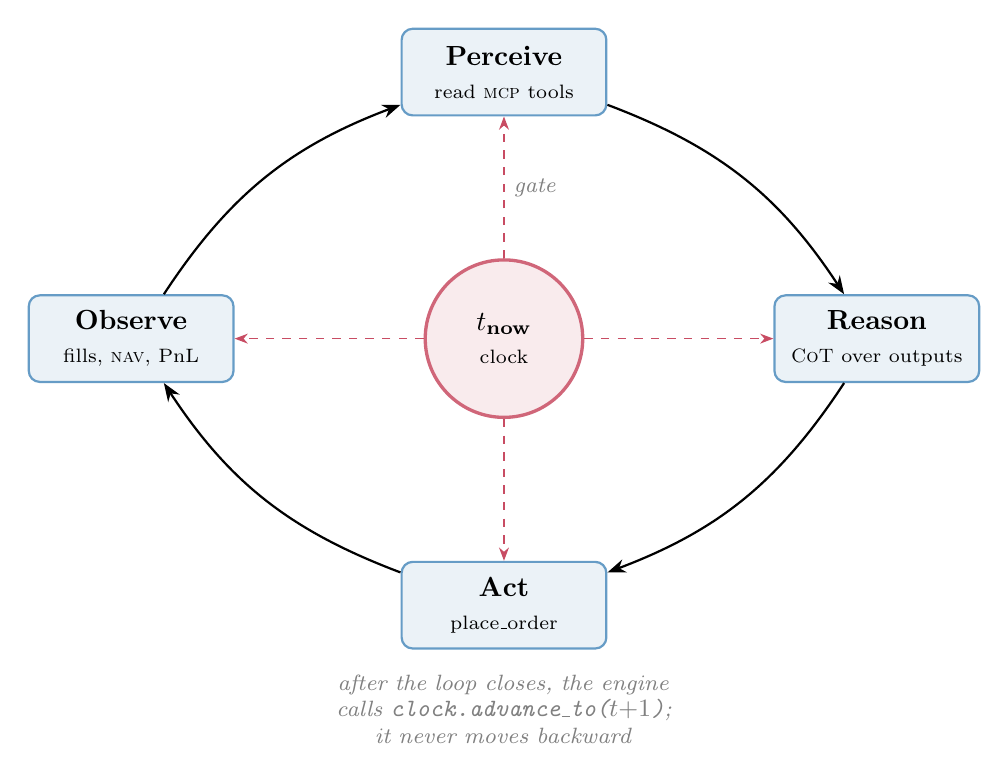
\begin{tikzpicture}[
      >=Stealth, node distance=20mm,
      stage/.style={draw, rounded corners, align=center, minimum width=26mm,
                    minimum height=11mm, fill=accent!8, draw=accent!60, thick},
      clk/.style={draw, circle, align=center, minimum size=20mm, fill=todored!8,
                  draw=todored!60, very thick},
      lbl/.style={font=\footnotesize\itshape, text=gray}
    ]
    \node[clk] (clock) {\textbf{\tnow}\\\scriptsize clock};

    \node[stage, above=18mm of clock]            (perceive) {\textbf{Perceive}\\\scriptsize read \mcp\ tools};
    \node[stage, right=24mm of clock]            (reason)   {\textbf{Reason}\\\scriptsize \CoT\ over outputs};
    \node[stage, below=18mm of clock]            (act)      {\textbf{Act}\\\scriptsize place\_order};
    \node[stage, left=24mm of clock]             (observe)  {\textbf{Observe}\\\scriptsize fills, \nav, PnL};

    % outer cycle
    \draw[->, thick] (perceive) to[bend left=18] (reason);
    \draw[->, thick] (reason)   to[bend left=18] (act);
    \draw[->, thick] (act)      to[bend left=18] (observe);
    \draw[->, thick] (observe)  to[bend left=18] (perceive);

    % every tool read consults the clock
    \draw[->, dashed, todored!70] (clock) -- (perceive) node[midway, lbl, right]{gate};
    \draw[->, dashed, todored!70] (clock) -- (act);
    \draw[->, dashed, todored!70] (clock) -- (reason);
    \draw[->, dashed, todored!70] (clock) -- (observe);

    \node[lbl, below=2mm of act, text width=58mm, align=center]
      {after the loop closes, the engine calls \code{clock.advance\_to($t{+}1$)};
       it never moves backward};
  \end{tikzpicture}
  \caption[The clock-centred agent loop]{The \mbox{perceive\,$\rightarrow$\,reason\,$\rightarrow$\,act\,$\rightarrow$\,observe}
  loop executed once per bar per ticker. The simulation clock \tnow\ sits at the centre:
  every data read (dashed arrows) is gated by it, so the agent can never perceive a
  datapoint dated after \tnow. The same loop runs in backtest and in live operation; only
  the clock's advance source differs (event loop versus wall clock). After the loop closes,
  the engine advances the clock strictly forward, which is the only mutation that exposes
  new data.}
  \label{fig:loop}
\end{figure}


This is the thesis's central methodological claim, and it is worth stating precisely.

\begin{invariant}[No look-ahead]
\label{inv:nolookahead}
For any data tool $T$ invoked while the clock reads \tnow, every item $x$ in $T$'s output
satisfies $\textsf{timestamp}(x) \le \tnow$. The bar timestamped exactly \tnow\ is
included; the first future bar is excluded. The inequality is \emph{strict} on the future
side.
\end{invariant}

The boundary semantics matter. A daily bar dated \tnow\ represents information known at the
close of that trading day, which is precisely the agent's decision point; it must be
visible. The next bar must not be. \Cref{fig:clockflow} illustrates the read path and the
strict boundary.

% ---------------------------------------------------------------------
% Figure: clock-gated data flow. raw cache -> t_now filter -> tool ->
% agent, contrasting an included past bar with an excluded future bar.
% ---------------------------------------------------------------------
\begin{figure}[t]
  \centering
  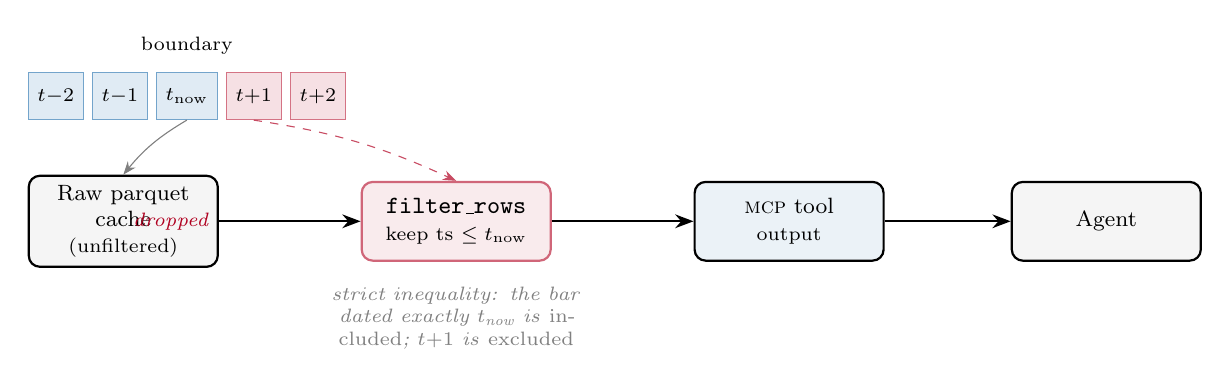
\begin{tikzpicture}[
      >=Stealth, font=\footnotesize, node distance=14mm,
      box/.style={draw, rounded corners, align=center, minimum height=10mm,
                  minimum width=24mm, thick},
      bar/.style={draw, minimum width=7mm, minimum height=6mm, font=\scriptsize},
      pass/.style={fill=accent!12, draw=accent!55},
      drop/.style={fill=todored!12, draw=todored!55},
    ]
    \node[box, fill=gray!8] (cache) {Raw parquet\\cache\\\scriptsize (unfiltered)};
    \node[box, fill=todored!8, draw=todored!60, right=18mm of cache] (filter)
      {\code{filter\_rows}\\\scriptsize keep ts $\le\tnow$};
    \node[box, fill=accent!8, right=18mm of filter] (tool) {\mcp\ tool\\\scriptsize output};
    \node[box, fill=gray!8, right=16mm of tool] (agent) {Agent};

    \draw[->, thick] (cache) -- (filter);
    \draw[->, thick] (filter) -- (tool);
    \draw[->, thick] (tool) -- (agent);

    % illustrative bars above the cache
    \node[bar, pass, above=10mm of cache.north west, anchor=west] (b1) {$t{-}2$};
    \node[bar, pass, right=1mm of b1] (b2) {$t{-}1$};
    \node[bar, pass, right=1mm of b2] (b3) {$\tnow$};
    \node[bar, drop, right=1mm of b3] (b4) {$t{+}1$};
    \node[bar, drop, right=1mm of b4] (b5) {$t{+}2$};
    \node[font=\scriptsize, above=1mm of b3] {boundary};

    \draw[->, gray] (b3.south) to[bend right=10] (cache.north);
    \draw[->, todored!70, dashed] (b4.south) to[bend left=8] (filter.north)
      node[midway, right, font=\scriptsize\itshape, text=todored]{dropped};

    \node[font=\scriptsize\itshape, text=gray, below=2mm of filter, text width=42mm,
          align=center]
      {strict inequality: the bar dated exactly \tnow\ is \emph{included}; $t{+}1$ is
       \emph{excluded}};
  \end{tikzpicture}
  \caption[Clock-gated data flow]{The clock-gated read path. Data is cached raw and never
  pre-trimmed; the \tnow\ filter is applied at read time inside the data wrapper. The
  invariant is a strict inequality --- the bar timestamped exactly \tnow\ is returned, the
  first future bar ($t{+}1$) is dropped --- so the agent sees ``the world as of the close of
  \tnow'' and nothing later. The single-item variant \code{assert\_not\_future} \emph{raises}
  instead of dropping, for cases where a future timestamp is unambiguously a bug.}
  \label{fig:clockflow}
\end{figure}


\subsection{Two enforcement modes}

The clock exposes two complementary guards, reflecting two genuinely different situations:

\begin{itemize}
  \item \code{filter\_rows(rows, date\_key)} --- the \emph{batch} guard. It returns only
  the rows with timestamp $\le\tnow$ and silently drops the rest. This is the expected,
  routine operation when slicing a cached price series to the visible window: future rows
  in the cache are not a bug, they are simply not yet visible. Dropping them is the correct
  behaviour.
  \item \code{assert\_not\_future(ts, label)} --- the \emph{single-item} guard. It
  \emph{raises} \code{FutureDataError} if \code{ts} is strictly after \tnow. This is used
  where a future timestamp is unambiguously a defect rather than an expected trim --- for
  instance, when an execution fill is stamped with a date the engine should never have
  reached.
\end{itemize}

Both guards route through one internal comparison, and both fail loudly rather than
returning a silent default. This reflects a project-wide convention: a silent fallback that
masks a leak or a missing tool call is the worst possible bug in a thesis whose entire
credibility rests on the absence of look-ahead. The codebase therefore raises on unexpected
states everywhere in the data path.

\subsection{Caching discipline that preserves the guarantee}

Performance requires caching market data to disk (parquet) so that a backtest is
re-runnable offline at zero API cost. Naively, caching and the temporal guarantee are in
tension: a cache populated by one run could expose future data to another. We resolve this
by \emph{caching raw data and applying the \tnow\ filter at read time}, never at write time.
A single parquet file is therefore valid for a run at any clock position: the same AAPL
cache serves a decision at \tnow${}={}$2023-01-03 and one at 2023-01-04, because the filter,
not the file, defines what is visible. This is shown as the substrate in
\cref{fig:architecture}.

\subsection{Timestamp normalisation}

A subtle correctness hazard is timezone handling. Comparing a timezone-aware news timestamp
against a naive \tnow\ can misplace items across the boundary by up to a day. We normalise
all timestamps to a single internal convention --- UTC-naive --- and, crucially, convert
aware datetimes to UTC \emph{before} stripping the offset. A bare offset-strip would, for
example, treat a Tokyo \texttt{+09:00} item as nine hours later than its true UTC instant,
which can flip a past item into an apparent future one and trigger a spurious leak (or, in a
filter context, an erroneous drop). The conversion is exercised in both boundary directions
by dedicated tests.

\section{Test-driven anti-leakage and mutation testing}
\label{sec:tdd}

The invariant in \cref{inv:nolookahead} is only as credible as the tests that enforce it.
Following the project's TDD mandate, the anti-look-ahead tests were written \emph{before}
the data layer they guard: \file{tests/test\_clock\_no\_lookahead.py} and
\file{tests/test\_data\_temporal\_filter.py}. They assert, among other properties, that a
tool returning a bar dated after \tnow\ causes a test failure --- which means the test
suite is red until the filter is correctly in place. These tests are treated as
non-negotiable: they are never weakened to make code pass.

Passing a hand-written test, however, only shows that the guard works on the cases the
author thought to write. To argue that the guard is \emph{load-bearing} --- that removing or
weakening it would actually be caught --- we use mutation testing as a falsification check.
Mutating the boundary comparison (for example, relaxing the strict future-side inequality
\code{>} to \code{>=}, or inverting the filter predicate) must cause at least one test to
fail. A surviving mutant would indicate a guard that is not actually exercised, which for
this particular invariant is a methodological red flag rather than a mere coverage gap. The
strict-versus-non-strict boundary is explicitly pinned this way.

\section{Leakage channels a temporal filter does not close}
\label{sec:leakage}

\Cref{inv:nolookahead} closes the \emph{when} of leakage. Two further channels concern the
\emph{what} and were the source of real, diagnosed bugs in this project; they are treated
honestly here rather than glossed over.

\subsection{Adjusted-price leakage}

Split- and dividend-adjusted price histories encode \emph{future} corporate actions into
past prices, because the adjustment factors are computed from the current state of the
world. A backtest set in 2022 that reads 2022 prices adjusted for a 2023 split is, subtly,
looking ahead. We therefore source \emph{unadjusted} prices throughout
(\code{auto\_adjust=False}) and work with raw OHLCV. The cost is that long-horizon return
comparisons are not split-corrected; this is the strictly preferable trade-off, because the
alternative is silent contamination of exactly the kind the thesis claims to prevent. The
choice is documented in the decision log.

A related, harder lesson from this project is that temporal correctness does not imply
\emph{value} correctness. An early run was corrupted not by look-ahead but by a data-handling
defect: a single-ticker download returned a column structure that, when indexed naively,
yielded a multi-element series where a scalar close price was expected, and a permissive
exception handler silently accepted malformed bars. The anti-look-ahead fortress checked
\emph{when} a bar was dated but never \emph{what} it contained. The response was a
fail-loud data-sanity gate (\file{bar\_validation.py}) that rejects non-scalar, non-finite,
non-positive, or internally inconsistent bars (e.g. high $<$ low, or a close outside a
plausible band around the open), together with a price-continuity guard that raises on
adjacent-bar jumps beyond a fixed ratio. These checks run on both the write and read paths,
so a previously cached corrupt bar is caught on first access. This episode is revisited as
part of the rigour narrative in \cref{sec:rigour}.

\subsection{Weight-memory contamination}

The most intractable channel is that the model's parameters already encode the approximate
outcome of historical events. A model trained on data through early 2025 ``knows,'' in a
diffuse statistical sense, how 2022--2024 unfolded; it can in principle infer future prices
from recalled news even when no future datum is served. KellyBench frames this directly: a
real news corpus does not eliminate the risk --- it only makes the grounding metric
meaningful, by giving cited claims something verifiable to check against.

We mitigate, and otherwise document honestly, rather than claim to solve:
\begin{enumerate}
  \item the agent is instructed to follow a rule-based process over tool outputs, reducing
  reliance on free recall;
  \item where feasible the test window is pushed toward, or past, the model's training
  cutoff, so that recall is less informative;
  \item the limitation is stated plainly as a threat to validity in \cref{sec:limitations},
  in the spirit of KellyBench's own candour.
\end{enumerate}
This honesty is itself a graded virtue: a thesis that names the channel it cannot fully
close is more credible than one that pretends the channel does not exist.

\section{Market-regime labelling}
\label{sec:regime}

Every downstream metric --- financial and reasoning alike --- is segmented by market
regime, because the thesis's substantive question is not ``can the agent trade?'' but
``\emph{when}, and \emph{why}, does it trade well or badly?''. This requires a regime
labelling that is itself causal: a label at bar $t$ must depend only on data up to $t$.

\subsection{Why rule-based, not HMM}

A hidden Markov model would give probabilistic regime assignments but requires fitting
transition parameters on historical data; done naively on the full series, that fit leaks
future information into past labels. We use instead a rule-based labelling from realised
volatility and trend, with thresholds fixed before seeing the data. It is less elegant than
an HMM but fully causal at every bar, which is the property the thesis needs; the HMM is
noted as future work.

\subsection{The detector}

The labelling (\file{mcp\_servers/analytics/regime.py}) assigns one of four labels with the
priority order \textsc{high\_vol} $>$ \textsc{bull} $>$ \textsc{bear} $>$ \textsc{range}.
The current detector (v2) improves on an initial version (v1) in two ways that are both
causality fixes:
\begin{itemize}
  \item \textbf{Reactive trend.} The bull/bear signal uses a short, 20-trading-day trend
  window ($\pm 2\%$ threshold), roughly one calendar month. The earlier 60-day window
  systematically lagged the 2022--2023 recovery, keeping a stale bearish label for weeks
  after prices had turned. The shorter window pivots about a month earlier at recovery
  inflections.
  \item \textbf{Causal volatility threshold.} The \textsc{high\_vol} label fires when
  realised volatility exceeds a trailing 252-bar percentile. The earlier version used a
  full-series percentile, which is a look-ahead: a future volatility spike would raise the
  threshold and silently re-label past bars when the series was extended. The trailing
  percentile uses only bars up to $t$. A dedicated test fails if a full-series percentile is
  reintroduced.
\end{itemize}

\subsection{Smoothing and warm-up}

Raw labels flip too often to support meaningful segmentation: a large fraction of regime
runs would otherwise last a single bar. We apply a causal minimum-hold smoothing (default
three bars, one trading week): a regime change is confirmed only after the new label has
persisted for the hold length. The smoothing is one-sided in time --- the smoothed label at
$t$ depends only on raw labels up to $t$ --- and a test verifies this anti-look-ahead
property explicitly. The raw label is retained as a diagnostic field.

The detector also imposes a hard warm-up requirement, derived rather than guessed. The
controlling constraint is the volatility-percentile window: for bar $t$ to have a
fully-populated trailing window, $t$ must be at least
$\textsf{vol\_window} + \textsf{vol\_percentile\_window} - 1 = 20 + 252 - 1 = 271$ trading
days into the data. The data window for any run therefore extends the decision window
backward by \code{REGIME\_WARMUP\_TRADING\_DAYS}${}=271$ trading days
(\code{REGIME\_WARMUP\_CALENDAR\_DAYS}${}=420$ calendar days with a safety margin). Both
backtest engines import this single constant, and an anti-regression test fails if it is set
too small or if the percentile window is changed without realigning it --- so that the
warm-up cannot silently drift out of sync with the detector. This guarantees that the first
\emph{decision} bar already has a correctly-initialised regime label, and that no decision
is excluded as warm-up.

\section{Baselines}
\label{sec:baselines}

An agent's performance is meaningless without a systematic yardstick, and the yardstick must
be at least as carefully constructed as the agent. We implement three baselines
(\file{backtest/baselines.py}): equal-weight Buy-\&-Hold, time-series momentum, and
Bollinger-band mean-reversion. Two properties make the comparison fair.

\paragraph{One-bar signal shift.} Every baseline signal is computed from the close of bar
$t$ and executed at bar $t{+}1$ (\code{exec\_signal = signal.shift(1)}). Same-bar execution
would let a baseline trade on a close it could not yet have known --- the baselines' own
look-ahead. A test fails if the shift is removed, mirroring the structural discipline applied
to the agent.

\paragraph{Symmetric transaction costs.} Costs were, in an earlier iteration, asymmetric ---
the agent paid nothing while the baselines paid a round-trip friction --- which silently
invalidated any comparison. We now charge $5$\,bps commission plus $5$\,bps slippage
($10$\,bps one-way) to \emph{both} the agent and the baselines, with Buy-\&-Hold charged an
entry and an exit cost. A test asserts cost symmetry on every run. We additionally report
turnover and a \emph{cost drag} (total commission as a fraction of initial \nav, in bps), so
that a high-turnover strategy's frictional cost is visible rather than buried in the net
return.

The baselines are computed vectorised in pandas, which is sufficient for daily data at this
scale; the event-driven engine is reserved for the agent path, where bar-by-bar drip-feed
realism matters. The decision to use pandas rather than a heavier vectorised backtester is
recorded in the decision log and turns on readability, not performance.

\section{Quantifying uncertainty: bootstrap confidence intervals}
\label{sec:bootstrap}

A single Sharpe number from a single run proves little; KellyBench shows single-seed
estimates can vary widely. We therefore report a bootstrap confidence interval around the
Sharpe ratio (\code{bootstrap\_sharpe\_ci} in \file{eval/financial.py}), resampling daily
returns to form the interval. Two honest caveats apply.

First, we use an \emph{i.i.d.}\ bootstrap rather than the stationary bootstrap of
Politis and Romano~\cite{politis1994}. Daily equity returns have weak autocorrelation, so
the i.i.d.\ resample is a reasonable approximation, but for a strategy with genuine momentum
the interval width may be mildly understated. The stationary bootstrap is the principled
upgrade and is flagged as such.

Second, the interval is only meaningful with enough \nav\ points: on a very short window the
resampled distribution degenerates and the interval collapses to a point. We treat
\minNavPoints\ daily \nav\ points as the minimum for a reportable interval, and we
\emph{never} annualise a Sharpe ratio computed on a short window --- annualising a Sharpe
estimated over, say, nineteen trading days inflates a noisy monthly figure into a
meaningless headline number. The full-period run is what supplies the thesis's confidence
interval; short windows are used only for plumbing validation and are labelled as such.

\section{Run scale tiers and reproducibility}
\label{sec:tiers}

LLM experiments cost real money, so every run declares a \emph{tier} (\file{backtest/tier.py})
that bounds its size before any model is called: \textsc{smoke} (development and CI, no cost
acknowledgement), \textsc{medium} (first real per-regime validation, up to about one month),
and \textsc{full} (explicit thesis-scale runs). All tiers enforce the regime warm-up. Every
result in this thesis is labelled with its scope: the older two-year single-agent run supports
the primary reasoning diagnosis, while the one-year common-reference run supplies the clean
cost-symmetric comparison. Development uses the cheapest capable model with cached responses
keyed by prompt hash, so debugging re-runs cost nothing and thesis-scale runs are executed only
after dry-run guardrails and data-cache preflight pass.

\chapter{System Architecture}
\label{ch:architecture}

This chapter describes the system that sits on top of the methodological substrate of
\cref{ch:methodology}. We move from the layered view (\cref{sec:layers}) through the
\mcp\ tool servers (\cref{sec:servers}), the single-agent orchestrator that is the thesis's
\emph{primary} result (\cref{sec:single}), the Portfolio-Manager multi-agent extension that
is reported as a \emph{bonus} (\cref{sec:pm}), the news corpus and its causal design
(\cref{sec:news}), and the observability layer that feeds the evaluation
(\cref{sec:observability}). Throughout, we are explicit about what is on the critical path
and what is not, because that hierarchy is itself part of the contribution: the thesis is
graded on evaluation rigour, and the architecture is sequenced to protect it.

% ---------------------------------------------------------------------
% Figure: layered architecture. MCP servers (data / analytics /
% execution) -> agent orchestrator -> evaluation harness, all sitting on
% the clock substrate.
% ---------------------------------------------------------------------
\begin{figure}[t]
  \centering
  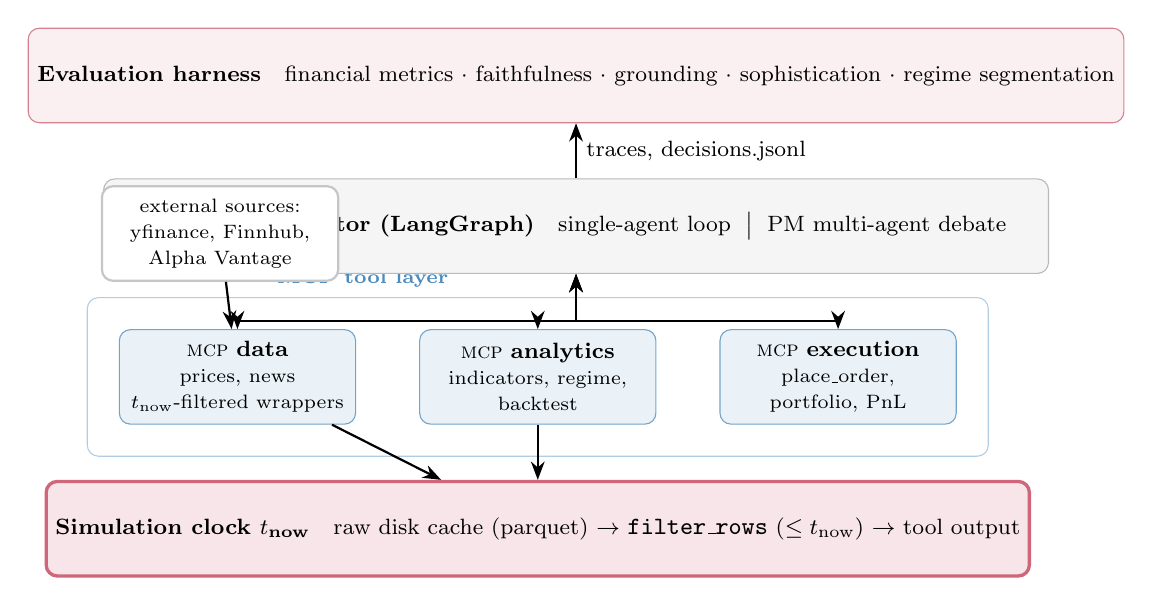
\begin{tikzpicture}[
      >=Stealth, font=\footnotesize,
      layer/.style={draw, rounded corners, align=center, minimum height=12mm,
                    thick},
      srv/.style={draw, rounded corners, align=center, minimum width=30mm,
                  minimum height=12mm, fill=accent!8, draw=accent!55},
      band/.style={draw, rounded corners, align=center, minimum width=120mm,
                   minimum height=12mm},
    ]
    % evaluation (top)
    \node[band, fill=todored!6, draw=todored!50] (eval)
      {\textbf{Evaluation harness}\quad financial metrics $\cdot$ faithfulness $\cdot$ grounding $\cdot$ sophistication $\cdot$ regime segmentation};

    % agent layer
    \node[band, below=7mm of eval, fill=gray!8, draw=gray!55] (agent)
      {\textbf{Agent orchestrator (LangGraph)}\quad single-agent loop \;$\big|$\; PM multi-agent debate};

    % MCP server row
    \node[srv, below=7mm of agent.south west, anchor=north west, xshift=2mm] (data)
      {\mcp\ \textbf{data}\\\scriptsize prices, news\\\scriptsize \tnow-filtered wrappers};
    \node[srv, right=8mm of data] (analytics)
      {\mcp\ \textbf{analytics}\\\scriptsize indicators, regime,\\\scriptsize backtest};
    \node[srv, right=8mm of analytics] (exec)
      {\mcp\ \textbf{execution}\\\scriptsize place\_order,\\\scriptsize portfolio, PnL};

    % clock substrate (bottom)
    \node[band, below=7mm of analytics, fill=todored!10, draw=todored!60, very thick,
          minimum width=120mm] (clock)
      {\textbf{Simulation clock \tnow}\quad raw disk cache (parquet) $\rightarrow$ \code{filter\_rows} ($\le\tnow$) $\rightarrow$ tool output};

    % external data behind data server
    \node[layer, above left=6mm and -28mm of data, fill=white, draw=gray!45,
          minimum width=30mm] (ext)
      {\scriptsize external sources:\\\scriptsize yfinance, Finnhub,\\\scriptsize Alpha Vantage};

    % arrows
    \draw[->, thick] (agent) -- (eval) node[midway, right]{traces, decisions.jsonl};
    \draw[<->, thick] (agent.south) -- ++(0,-6mm) -| (data.north);
    \draw[<->, thick] (agent.south) -- ++(0,-6mm) -| (analytics.north);
    \draw[<->, thick] (agent.south) -- ++(0,-6mm) -| (exec.north);
    \draw[->, thick] (data) -- (clock);
    \draw[->, thick] (analytics) -- (clock);
    \draw[->, thick] (ext) -- (data);

    \begin{scope}[on background layer]
      \node[draw=accent!30, rounded corners, fit=(data)(analytics)(exec),
            inner sep=4mm, label={[accent!70,font=\scriptsize\bfseries]above left:MCP tool layer}] {};
    \end{scope}
  \end{tikzpicture}
  \caption[Layered system architecture]{Layered architecture. External data sources enter
  only through \mcp\ \emph{data} wrappers that enforce the \tnow\ filter; the \emph{analytics}
  and \emph{execution} servers expose indicators/regime/backtest and paper-trading
  respectively. The orchestrator composes these heterogeneous servers --- the core premise of
  the thesis topic --- and emits one structured decision record per step. The evaluation
  harness consumes those records. The clock substrate underlies every read: data is cached
  raw and filtered to $\le\tnow$ at read time, so a single cache file is reusable across
  runs at different clock positions.}
  \label{fig:architecture}
\end{figure}


\section{Layered overview}
\label{sec:layers}

\Cref{fig:architecture} shows four layers. At the base is the clock substrate of
\cref{sec:timemachine}: raw cached data filtered to $\le\tnow$ at read time. Above it sit
three \mcp\ servers --- \emph{data}, \emph{analytics}, and \emph{execution} --- each a
narrow, typed surface. Above those, the agent orchestrator composes the servers in its
reasoning loop. At the top, the evaluation harness consumes the structured decision records
the orchestrator emits. The key architectural premise, and the one that matches the thesis
topic, is that the agent reaches \emph{all} capabilities --- market data, indicators,
sentiment, portfolio state, execution --- only through \mcp\ tool calls, never through
in-process shortcuts. This is what makes the backtest/live equivalence exact: the same tool
calls, the same server code, only a different clock.

\section{The MCP tool servers}
\label{sec:servers}

\subsection{Data server}

The data server wraps external sources (yfinance for prices, Finnhub and Alpha Vantage for
news) behind tools that enforce \cref{inv:nolookahead}. Its tools expose price history,
news items, and derived metadata; each filters its output through the clock before
returning. Crucially, the wrapper --- not the external source --- owns the temporal
guarantee, so swapping or adding a data provider does not move the choke point. The decision
to wrap rather than re-implement external \mcp\ data servers reflects the topic's intent:
the agent composes heterogeneous \mcp\ servers, and the thesis's own server exposes only
what is thesis-specific.

\subsection{Analytics server}

The analytics server exposes custom technical indicators, the regime detector of
\cref{sec:regime}, and backtest utilities. Indicators are precomputed once per dataset and
read through the tool, rather than recomputed every bar, so the hot path stays light. The
indicator and sentiment formulas were adapted from the supervisor's reference teaching
code, re-implemented in our codebase with type annotations, tests, and the temporal filter
rather than imported wholesale.

\subsection{Execution server}

The execution server is an in-memory paper-trading broker: \code{place\_order},
\code{get\_portfolio}, \code{get\_pnl}. It accepts an explicit price parameter rather than
looking up a price internally, which keeps it independent of the data server (no circular
dependency) and makes the price assumption explicit and traceable in every decision record.
It enforces the portfolio constraints structurally: long-only, no leverage, non-negative
cash, and a hard per-position cap. The cap is enforced at order time by clamping the
requested quantity \emph{down} to the admissible maximum --- never up --- a direction that,
when once inverted, was the cause of a catastrophic early run and is now both fixed and
tested (\cref{sec:rigour}).

\section{Single-agent orchestrator (primary result)}
\label{sec:single}

The single-agent system is the thesis's primary, canonical result. It is a minimal
LangGraph~\cite{langgraph2024} graph implementing the loop of \cref{fig:loop}: a small,
explicit, typed state object flows through perceive, reason/act, and observe nodes, with the
clock advancing once per step. LangGraph is used here in its canonical tutorial shape ---
\code{StateGraph}, nodes, conditional edges, checkpointing --- deliberately on the simplest
possible surface, so that the framework is learned \emph{off} the evaluation critical path.
The decision to introduce LangGraph in this order, rather than starting with a complex
multi-agent graph, is recorded in the decision log as a risk-management choice.

\subsection{Sizing policy and why it matters for evaluation}

The agent operates a simple, explicit position-sizing policy, stated in its system prompt: a
base target of $10\%$ of \nav\ per position, a high-conviction target of $15\%$, and a hard
cap of $20\%$. This policy is not incidental --- it is the reference against which
faithfulness is judged (\cref{sec:faithfulness}). A judge that did not know the policy would
mistake a deliberate hold at the $10\%$ target for a reasoning failure; encoding the policy
into the judge is precisely the fix that distinguishes the v1 and v2 judges.

\subsection{Decision record schema}

After each step the orchestrator writes one JSON line to \file{decisions.jsonl}, flushed
immediately so that a crash never loses a paid-for decision. The record captures both halves
of what the reasoning metrics need: the \emph{stated} side (full chain-of-thought rationale,
intended action) and the \emph{actual} side (the executed order and fill, the regime label,
the flattened indicator values, and the raw tool outputs the agent saw). Recording the raw
tool outputs --- recent OHLCV bars, the indicator dictionary, the portfolio snapshot with
each position's percentage of \nav\ --- is what makes grounding verifiable: a claim in the
prose can be checked against the number the tool actually returned. This dual capture is the
schema-level reason the faithfulness and grounding metrics are well-defined.

\subsection{Asynchronous execution without breaking determinism}

The per-bar loop issues one LLM call per ticker. To keep wall-clock time tractable, calls
within a single date are dispatched concurrently under a bounded semaphore, but all tickers
on a date are scored against the \emph{same} start-of-date portfolio snapshot, and orders
are then executed serially in a deterministic ticker order. A non-regression test asserts
that the concurrent path produces byte-identical decisions to a serial run, so concurrency
is a pure latency optimisation with no effect on results. Transient API errors are retried
with exponential back-off; this, and a token-budget fix, were prerequisites for the long run
to complete at all (\cref{sec:rigour}).

\section{Portfolio-Manager multi-agent extension (bonus)}
\label{sec:pm}

The multi-agent Portfolio Manager (PM) is reported honestly as a \emph{bonus} on top of the
single-agent result, not as a prerequisite. This hierarchy follows directly from the
project's evaluation-first principle and from the finding of Agent Market
Arena~\cite{ama2025} that architecture matters more than backbone: the interesting question
is whether deliberation changes \emph{behaviour}, specifically whether it closes the
single-agent's exit-discipline gap. \Cref{fig:pmpipeline} shows the pipeline.

% ---------------------------------------------------------------------
% Figure: PM multi-agent pipeline (TradingAgents-style communication
% topology): analysts -> bull/bear debate -> research manager -> trader
% -> risk debate -> PM weights -> memory log.
% ---------------------------------------------------------------------
\begin{figure}[t]
  \centering
  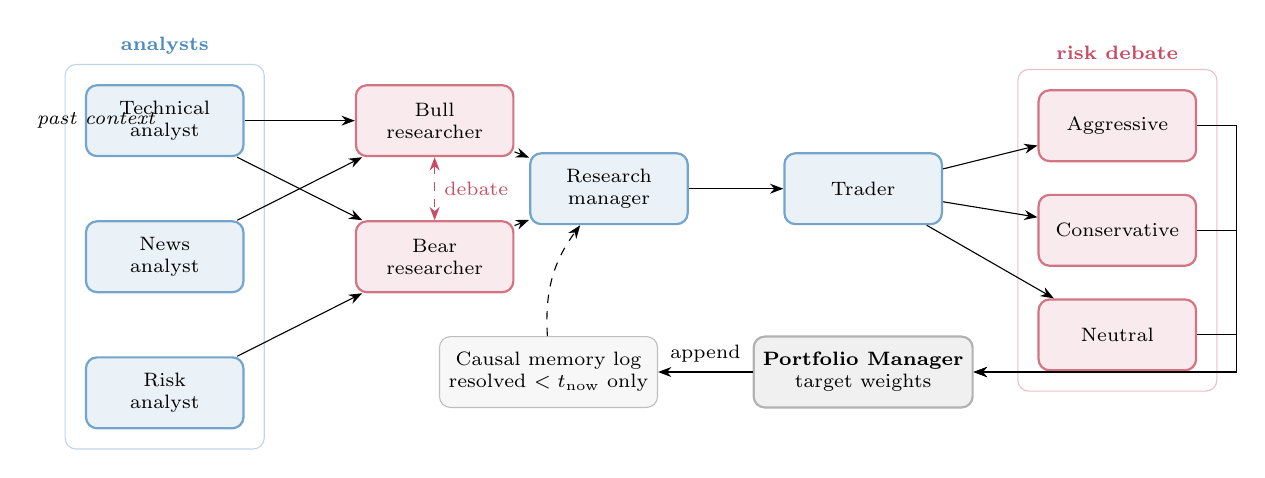
\begin{tikzpicture}[
      >=Stealth, font=\scriptsize, node distance=8mm and 11mm,
      n/.style={draw, rounded corners, align=center, minimum height=9mm,
                minimum width=20mm, thick, fill=accent!8, draw=accent!55},
      deb/.style={n, fill=todored!8, draw=todored!55},
      pm/.style={n, fill=gray!12, draw=gray!60, minimum width=26mm},
      mem/.style={draw, rounded corners, align=center, minimum height=9mm,
                  fill=gray!6, draw=gray!50, minimum width=26mm},
    ]
    % analysts column
    \node[n] (tech) {Technical\\analyst};
    \node[n, below=of tech] (news) {News\\analyst};
    \node[n, below=of news] (risk) {Risk\\analyst};

    % debate
    \node[deb, right=14mm of tech] (bull) {Bull\\researcher};
    \node[deb, below=of bull] (bear) {Bear\\researcher};
    \node[n, right=12mm of {$(bull)!0.5!(bear)$}] (rm) {Research\\manager};

    \node[n, right=12mm of rm] (trader) {Trader};

    % risk debate
    \node[deb, right=12mm of trader, yshift=8mm] (agg) {Aggressive};
    \node[deb, below=4mm of agg] (con) {Conservative};
    \node[deb, below=4mm of con] (neu) {Neutral};

    \node[pm, below=14mm of trader] (pm) {\textbf{Portfolio Manager}\\target weights};
    \node[mem, left=12mm of pm] (memlog) {Causal memory log\\\scriptsize resolved $<\tnow$ only};

    % flows
    \draw[->] (tech) -- (bull);
    \draw[->] (news) -- (bull);
    \draw[->] (risk) -- (bear);
    \draw[->] (tech) -- (bear);
    \draw[<->, dashed, todored!70] (bull) -- (bear) node[midway, right]{debate};
    \draw[->] (bull) -- (rm);
    \draw[->] (bear) -- (rm);
    \draw[->] (rm) -- (trader);
    \draw[->] (trader) -- (agg);
    \draw[->] (trader) -- (con);
    \draw[->] (trader) -- (neu);
    \draw[->] (agg.east) -- ++(5mm,0) |- (pm.east);
    \draw[->] (con.east) -- ++(5mm,0) |- (pm.east);
    \draw[->] (neu.east) -- ++(5mm,0) |- (pm.east);
    \draw[->] (pm) -- (memlog) node[midway, above, font=\scriptsize]{append};
    \draw[->, dashed] (memlog) to[bend left=20] (rm)
      node[midway, left, font=\scriptsize\itshape]{past context};

    \begin{scope}[on background layer]
      \node[draw=accent!25, rounded corners, fit=(tech)(news)(risk),
            inner sep=2.5mm, label={[font=\scriptsize\bfseries,accent!70]above:analysts}]{};
      \node[draw=todored!25, rounded corners, fit=(agg)(con)(neu),
            inner sep=2.5mm, label={[font=\scriptsize\bfseries,todored!70]above:risk debate}]{};
    \end{scope}
  \end{tikzpicture}
  \caption[Portfolio-Manager multi-agent pipeline]{The Portfolio-Manager (PM) multi-agent
  pipeline, adopting the \textsc{TradingAgents} communication topology re-implemented over
  our \mcp\ tool layer. Role analysts each see only their role-appropriate tool outputs (the
  news analyst, crucially, sees \emph{only} news items --- see \cref{sec:news}); a bounded
  Bull/Bear debate and a research manager synthesise a thesis; a trader proposes; a bounded
  Aggressive/Conservative/Neutral risk debate stress-tests it; and a single Portfolio
  Manager emits portfolio-level target weights, which a deterministic rebalancer turns into
  orders. A causal memory log feeds back only decisions resolved strictly before \tnow, so
  the deliberation never leaks future outcomes.}
  \label{fig:pmpipeline}
\end{figure}


\subsection{Communication topology}

The PM adopts the \textsc{TradingAgents}~\cite{tradingagents2024} communication topology:
role analysts (technical, news, risk) produce reports; a bounded Bull/Bear research debate
and a research manager synthesise an investment thesis; a trader proposes a position; a
bounded Aggressive/Conservative/Neutral risk debate stress-tests it; and a single Portfolio
Manager emits portfolio-level target weights. The cyclic debate is exactly the structure
that a hand-rolled loop handles awkwardly and a graph framework handles cleanly, which is
where LangGraph earns its place in the second phase rather than the first.

We adopt the \emph{contract} --- the role decomposition and the bounded message shape --- but
do not import third-party code: the topology is re-implemented over our \mcp\ tool layer
with compact JSON artifacts at each node instead of an unbounded chat transcript, so that the
cache, the decision schema, the rebalancer, and the evaluation plumbing remain unchanged. The
PM emits strict JSON parsed into a typed target-weight object; invalid JSON, negative weights,
unknown tickers, or implied leverage fail loudly at the parser boundary.

\subsection{Deterministic rebalancing and fail-loud errors}

Target weights are turned into orders by a \emph{deterministic} rebalancer, separating the
stochastic decision (the LLM allocation) from the mechanical execution (share counts under
the long-only, no-leverage, non-negative-cash constraints). A subtle but important
correctness property is that a PM API or parsing failure is tagged explicitly
(\code{is\_error}) and an all-cash fallback is written so the artifact is inspectable;
errored decisions are then excluded from every metric. Without this tag, a silent failure
would be indistinguishable from a legitimate all-cash allocation and would quietly pollute
the faithfulness tables.

\subsection{Causal memory}

The PM keeps an append-only memory log of past decisions and their later realised returns,
so that the deliberation can reference prior lessons in the manner of
\textsc{TradingAgents}. The log is gated by the clock: \code{get\_past\_context(t\_now)}
returns only entries whose decision date is strictly before \tnow\ \emph{and} whose outcomes
have already resolved, and the context is capped to the most recent entries to keep the
prompt bounded. This makes the memory a causal utility rather than a leakage channel: a
future outcome cannot enter a past deliberation by construction.

\section{News: a causally correct sentiment corpus}
\label{sec:news}

News sentiment is the data source where causal correctness is most fragile, and it is
treated as a \emph{feature} that is disabled by default rather than a load-bearing part of
the primary result. Two distinct risks shape the design.

\paragraph{Publication date versus event date.} A story about an earnings call (the event)
may be published before or after the call. Only the \emph{publication} timestamp
(\code{published\_at}) is observable to an agent at \tnow; filtering on the event date would
leak. The corpus and its clock filter therefore key strictly on \code{published\_at}.

\paragraph{Weight-memory contamination.} As in \cref{sec:leakage}, a real corpus does not
remove the model's latent knowledge of historical outcomes; it only makes the grounding
metric meaningful, by giving the news analyst's cited claims verifiable extracts to be
checked against. We state this limitation plainly rather than overclaim.

\paragraph{Corpus construction.} Candidate sources were evaluated on whether they expose a
true publication timestamp. Finnhub and Alpha Vantage do; a crawl-based source exposes only
crawl time and is therefore unsuitable as a primary timestamp. The corpus is built once,
cached to parquet, and filtered by \code{published\_at <= t\_now} at read time, exactly like
prices --- it is a static artifact, not a live scrape. A feature flag keeps the corpus off
by default; the primary single-agent result does not depend on it. We report the real state
honestly in \cref{ch:results}, including provider limitations encountered (a free Finnhub
plan that returned no rows for the older window, and a crawl key that failed locally).

\paragraph{Evidence discipline.} A diagnosed bug (\cref{sec:rigour}) had the news analyst
fabricating sentiment from technical indicators when no news was available. The fix has two
parts: the news analyst's prompt is restricted to \emph{only} news tool outputs (no
indicators, prices, or portfolio), and when no items exist for any ticker the LLM call is
skipped entirely in favour of a structured ``sentiment unavailable'' marker that contributes
zero weight to the consensus. Sentiment without a cited, timestamped extract is treated as
hallucination, not signal.

\section{Observability}
\label{sec:observability}

Every decision is traced to Langfuse Cloud~\cite{langfuse2024} as a structured object:
inputs seen, tool calls and their real outputs, the chain-of-thought, the resulting order,
latency, token count, and cost. We use Langfuse Cloud rather than self-hosting, since the
trace volume of a thesis is far below the free allowance and self-hosting would add
operational overhead for no benefit. OpenAI calls are traced via the SDK drop-in; PM
decisions emit a parent observation with child spans for each analyst, each debate stage, and
the final allocation, so the multi-agent structure is legible in the trace tree. The
reasoning metrics of \cref{ch:evaluation} consume the same captured inputs and outputs, and
the metric scores are attached back onto traces, which yields regime-segmented dashboards at
no extra cost. Trace export is best-effort: an export timeout never fails a local run, since
the authoritative artifact is the on-disk \file{decisions.jsonl}, not the trace.

\section{LLM backbone interface}
\label{sec:backbone}

The agents run on the OpenAI API behind a thin backbone interface, so that swapping or
adding a model --- for instance a second model for an architecture-versus-backbone
comparison in the spirit of~\cite{ama2025} --- is a localised change. In development the
backbone defaults to the cheapest capable model with a prompt-hash response cache, so that
re-runs during debugging cost nothing; the more expensive configuration is reserved for the
final run. A deterministic stub backbone exists for plumbing and CI, and any run using it is
labelled as such and is never cited as a thesis result.

\chapter{Evaluation Design}
\label{ch:evaluation}

The evaluation is the thesis's graded core, and this chapter defines it before any numbers
are reported. We cover the financial metrics and their regime segmentation
(\cref{sec:finmetrics}), then the three reasoning metrics --- faithfulness
(\cref{sec:faithfulness}), grounding (\cref{sec:grounding}), and sophistication
(\cref{sec:sophistication}) --- explaining in each case \emph{why} the chosen measurement
strategy fits the quantity. \Cref{sec:anchor} treats the judge--human anchoring that
underwrites the validity of the faithfulness metric. \Cref{sec:pmeval} extends the protocol
to the multi-agent path, and \cref{sec:rigour} presents the rigour narrative: the chain of
bugs caught, diagnosed, fixed, and tested. \Cref{fig:evalprotocol} summarises the protocol.

% ---------------------------------------------------------------------
% Figure: evaluation protocol. A logged decision fans out to three
% measurements: faithfulness (blind LLM judge), grounding (deterministic),
% and the human anchor that validates the judge.
% ---------------------------------------------------------------------
\begin{figure}[t]
  \centering
  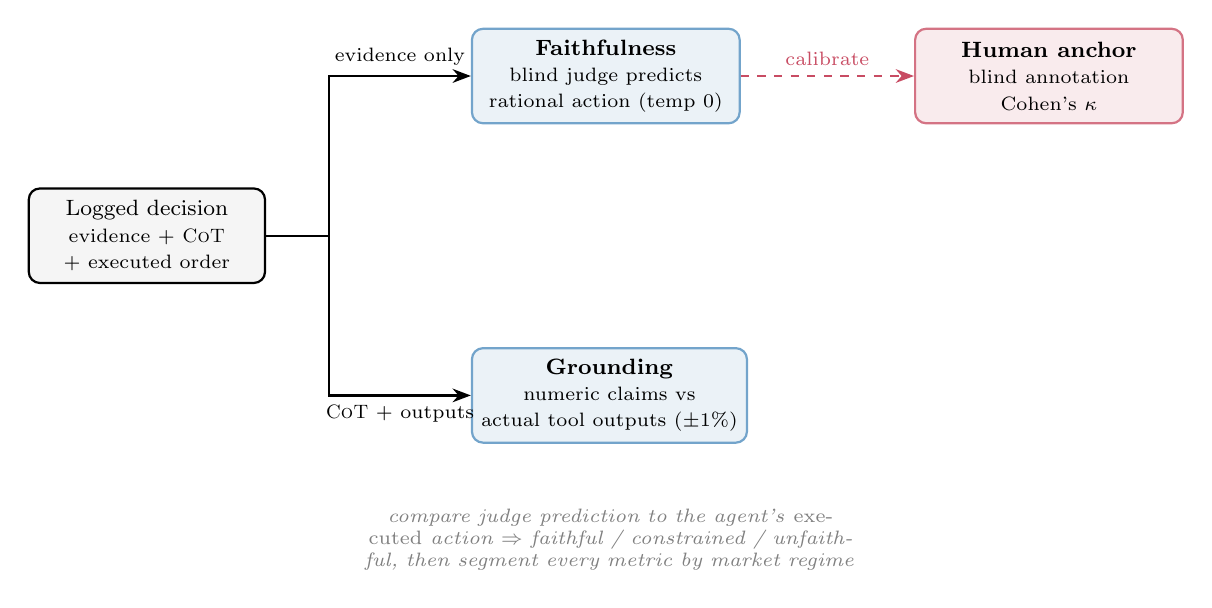
\begin{tikzpicture}[
      >=Stealth, font=\footnotesize, node distance=12mm,
      rec/.style={draw, rounded corners, align=center, minimum height=12mm,
                  minimum width=30mm, thick, fill=gray!8},
      m/.style={draw, rounded corners, align=center, minimum height=12mm,
                minimum width=34mm, thick},
      judge/.style={m, fill=accent!8, draw=accent!55},
      det/.style={m, fill=accent!8, draw=accent!55},
      hum/.style={m, fill=todored!8, draw=todored!55},
    ]
    \node[rec] (dec) {Logged decision\\\scriptsize evidence + \CoT\\\scriptsize + executed order};

    \node[judge, above right=8mm and 26mm of dec] (faith)
      {\textbf{Faithfulness}\\\scriptsize blind judge predicts\\\scriptsize rational action (temp 0)};
    \node[det, below right=8mm and 26mm of dec] (ground)
      {\textbf{Grounding}\\\scriptsize numeric claims vs\\\scriptsize actual tool outputs ($\pm1\%$)};

    \node[hum, right=22mm of faith] (human)
      {\textbf{Human anchor}\\\scriptsize blind annotation\\\scriptsize Cohen's $\kappa$};

    % what the judge sees vs what the agent did
    \draw[->, thick] (dec.east) -- ++(8mm,0) |- (faith.west)
      node[pos=0.75, above, font=\scriptsize]{evidence only};
    \draw[->, thick] (dec.east) -- ++(8mm,0) |- (ground.west)
      node[pos=0.75, below, font=\scriptsize]{\CoT\ + outputs};
    \draw[->, thick, dashed, todored!70] (faith) -- (human)
      node[midway, above, font=\scriptsize]{calibrate};

    \node[align=center, below=7mm of ground, text width=80mm, font=\scriptsize\itshape,
          text=gray]
      {compare judge prediction to the agent's \emph{executed} action $\Rightarrow$
       faithful / constrained / unfaithful, then segment every metric by market regime};
  \end{tikzpicture}
  \caption[Reasoning-evaluation protocol]{The reasoning-evaluation protocol. Each logged
  decision is measured along two automatic axes. \emph{Faithfulness} asks whether the
  executed trade matches the action a rational, policy-aware judge would take given
  \emph{only} the same objective evidence (regime, indicators, portfolio) --- deliberately
  withholding the agent's own rationale and action so the judge cannot simply echo them.
  \emph{Grounding} is deterministic: it extracts numeric claims from the chain-of-thought
  and checks each against the actual tool outputs within a $1\%$ tolerance. The judge is in
  turn anchored to blind human annotation (Cohen's $\kappa$), making the human agreement the
  validity cornerstone of the whole protocol. Every metric is finally segmented by regime.}
  \label{fig:evalprotocol}
\end{figure}


\section{Financial performance}
\label{sec:finmetrics}

Financial performance is reported against the baselines of \cref{sec:baselines} using a
standard risk-adjusted metric set computed in \file{eval/financial.py}: annualised return,
the Sharpe~\cite{sharpe1994} and Sortino~\cite{sortino1994} ratios, the Calmar ratio,
maximum drawdown, and hit rate, alongside turnover and cost drag. The metrics are pure
functions of the \nav\ series, which makes them trivially testable and cacheable. Each point
estimate is accompanied by the bootstrap confidence interval of \cref{sec:bootstrap}, and
the agent is compared on the \emph{same} window, the \emph{same} costs, and the \emph{same}
shift discipline as the baselines.

Crucially, financial performance is reported \emph{by regime}. A headline Sharpe that
aggregates a bull run with a high-volatility episode hides exactly the behaviour the thesis
is about. The regime labels of \cref{sec:regime} partition the decision sequence, and every
metric is recomputed within each partition. The expected --- and most interesting ---
finding is that performance and reasoning quality both degrade in adversarial regimes, in
line with ATLAS~\cite{atlas2025} and LiveTradeBench~\cite{livetradebench2025}.

\section{Faithfulness: the knowledge--action gap}
\label{sec:faithfulness}

\subsection{What it measures, and why a judge}

Faithfulness measures the knowledge--action gap of KellyBench~\cite{kellybench2026}: does the
agent \emph{do} what its reasoning implies it should do? The naive implementation --- parse
an intended action from the rationale and compare it to the executed action --- measures
almost nothing, because both fields are produced by the same LLM call and are trivially
self-consistent. Keyword extraction from the rationale is also fragile on nuanced prose
(``I will not sell yet'' misfires). The faithfulness signal we want is not internal
self-consistency but consistency between the agent's behaviour and what a \emph{rational
observer} would do on the same evidence.

We therefore use an independent LLM judge (temperature $0$ for determinism) that sees
\emph{only} the objective evidence the agent saw --- ticker, date, regime, technical
indicators, and the portfolio snapshot --- and predicts the rational action \emph{blind}: it
is shown neither the agent's rationale nor its executed action, so it cannot echo them. We
then compare the judge's prediction to the agent's actual executed action. This is the
reason faithfulness uses a judge while grounding does not (\cref{sec:grounding}):
faithfulness is an inherently judgemental counterfactual --- ``what \emph{should} a rational
agent have done here?'' --- whereas grounding is a factual check that has a deterministic
ground truth.

\subsection{Three verdicts}

Each scored decision receives one of three verdicts:
\begin{description}
  \item[Faithful] the agent's action matches what the policy-aware judge would do --- whether
  that is to trade or, deliberately, to hold.
  \item[Constrained] the agent could not have acted: a genuine \emph{capacity} constraint
  (e.g.\ cash below a minimal-trade threshold on the buy side, or a zero position on the
  sell side). These are excluded from the strict faithfulness denominator because they are
  not reasoning failures.
  \item[Unfaithful] a real gap: the judge predicts an action, the agent does not take it, and
  no capacity reason explains the difference.
\end{description}
The standard faithfulness rate counts faithful over all scoreable decisions; a
\emph{strict} variant additionally removes constrained decisions from the denominator. We
report both for comparability.

\subsection{Policy-awareness: the v1$\rightarrow$v2 redesign}
\label{sec:v2judge}

The first judge (v1) assumed a rational agent always deploys to the hard cap. This
systematically mislabelled deliberate holds at the $10$--$15\%$ target as unfaithful,
because the judge ``saw room to buy'' that the agent's own policy forbade using. The
correction (v2) makes the judge \emph{policy-aware}: it is told the base target ($10\%$),
the high-conviction target ($15\%$), and the hard cap ($20\%$), and that once a position is
at or above target, holding is the rational default unless a sell condition exists.

This redesign was \emph{pre-registered}: the policy specification and the verdict semantics
were locked, and validated by the author, \emph{before} the v2 numbers were computed. Locking
the metric definition before seeing its result is a direct response to KellyBench's warnings
about post-hoc metric tuning, and it is what lets us report the v1/v2 comparison as a
genuine methodological finding rather than a fit to a desired number. Both judges are kept in
the codebase behind a flag, and the thesis reports them side by side: v1 for comparison and
reproducibility, v2 as the canonical metric.

A structural consequence of policy-awareness is that the v2 judge resolves capacity cases
itself (it predicts ``hold'' for an at-cap or cash-starved position), so the explicit
constrained-override fires far less often --- the prompt does the work the override used to
do. The redesign also \emph{exposed} a finding the v1 judge had hidden: a class of
non-trimming decisions that v1 silently absorbed into ``constrained'' but v2 correctly marks
unfaithful. This is discussed quantitatively in \cref{ch:results}.

\section{Grounding: are the cited numbers real?}
\label{sec:grounding}

Grounding asks whether the numbers the agent cites in its reasoning are the actual outputs of
the tools it called, or hallucinations. Because this question has a deterministic ground
truth --- the tool outputs are recorded in the decision record --- it is computed
deterministically, with no LLM in the loop. A regex extracts \texttt{(label, value)} numeric
claims from the rationale; each claim is matched against the recorded indicator dictionary,
the recent OHLCV bars, or the portfolio snapshot within a $1\%$ relative tolerance. Grounding
is the fraction of claims that match. Decisions with no numeric claims score as ``no signal''
and are not penalised --- an unquantified rationale is not a hallucination.

The contrast with faithfulness is deliberate and is the methodological point of having both:
grounding is cheap, deterministic, and re-runnable for free on any decision file, so it
anchors the evaluation in a measurement that involves no model judgement at all; faithfulness
necessarily involves judgement and is therefore the metric that must be anchored to humans
(\cref{sec:anchor}). Reporting both protects against the failure mode where an agent cites
perfectly real numbers (high grounding) but acts against them (low faithfulness), which is
exactly the knowledge--action gap.

\section{Sophistication}
\label{sec:sophistication}

The third reasoning axis, planned in the manner of KellyBench's multi-point sophistication
rubric, scores a sampled subset of decisions on a small, explicit rubric --- risk
management, acknowledgement of uncertainty, regime adaptation, and coherence --- via an
LLM judge with structured output, sampled per regime to bound cost. Sophistication is the
most subjective of the three metrics and is reported as a planned, supporting measure rather
than a headline; its rubric maps directly onto the thesis claims about regime-adaptive
reasoning. Its results, where computed, are reported in \cref{ch:results} with the same
regime segmentation and the same candour about sampling.

\section{Anchoring the judge to humans}
\label{sec:anchor}

A metric computed by an LLM judge is only as trustworthy as its agreement with human
judgement; this anchoring is the validity cornerstone of the reasoning evaluation. We draw a
stratified sample of decisions, have them annotated blind against the same policy the judge
uses, and report the judge--human action agreement and Cohen's $\kappa$~\cite{cohen1960}.

Two points of rigour govern how the agreement is reported. First, the sample is
\emph{stratified} (deliberately over-sampling rare and diagnostic cases such as the
non-trimming class), not a representative random draw; we therefore report agreement
\emph{per stratum} and refrain from presenting a single global $\kappa$ as if the sample were
representative. If a population-level estimate is needed, a separate random sample must be
drawn. Second, a blind protocol is used for the medium-window reconciliation: annotations are
filled against sealed fields, and the key is opened only afterward, so the human labels
cannot be retrofitted to the judge. The per-stratum agreement, the global figures with their
representativeness caveat, and the blind-reconciliation result are all reported in
\cref{sec:resultsanchor}.

\section{Extending the protocol to the multi-agent path}
\label{sec:pmeval}

The PM path needs two adaptations. First, the regime label of a portfolio-level decision is
aggregated across its tickers by worst case (\textsc{high\_vol} $>$ \textsc{bear} $>$
\textsc{range} $>$ \textsc{bull}), so a portfolio decision inherits the most adverse regime
it faces. Second, faithfulness is redefined at the allocation level: for each
ticker after the first (baseline) decision, the PM's target-weight \emph{direction}
(increase/hold/decrease) is checked against the weighted analyst consensus, with the same
capacity-constraint exemptions (no cash to rebalance, already concentrated, cannot short from
zero).

Grounding also splits in two. The PM's final rationale is concise and often carries no
numeric claims, so the standard grounding metric can legitimately return ``no claims'' for
it --- which is not a failure. To audit the \emph{analysts'} evidence, a separate
\emph{evidence-grounding} metric checks each analyst's technical and risk claims against
indicators, bars, portfolio, and regime, and each news claim against the causal news tool
outputs by source and publication date. Finally, an artifact-level \emph{MCP time-machine
audit} sweeps the entire decision file for any tool output, order, or fill timestamped after
\tnow, and reports the per-source counts so that cache-versus-API provenance stays visible.
This audit is the empirical counterpart of \cref{inv:nolookahead}: it demonstrates, on the
completed artifact, that no future timestamp ever reached the agent.

\section{The rigour narrative: bugs caught, diagnosed, fixed, tested}
\label{sec:rigour}

This section is an argument, not a confession. A thesis whose central claim is methodological
rigour is strengthened, not weakened, by showing that its instruments \emph{caught} real
defects and that each defect was closed with a regression test. Each item below follows the
same shape: symptom $\rightarrow$ diagnosis $\rightarrow$ fix $\rightarrow$ test.

\begin{description}
  \item[Price-corruption masquerade.] An early run collapsed not from look-ahead but from a
  single-ticker download whose column structure yielded a non-scalar where a scalar close was
  expected; a permissive exception handler accepted the malformed bars silently. The
  anti-look-ahead tests checked \emph{when} a bar was dated, never \emph{what} it contained.
  \emph{Fix}: a fail-loud data-sanity gate (\file{bar\_validation.py}) plus a price-continuity
  guard rejecting implausible adjacent-bar jumps, on both write and read paths. \emph{Test}:
  a suite that reproduces the exact failure mode (multi-element series) and a cache-read
  regression guard.
  \item[Engine cap inverted.] A position-cap clamp set the order quantity \emph{up} to the
  cap rather than \emph{down}, inflating small legitimate orders to the ceiling and destroying
  the portfolio. \emph{Fix}: clamp strictly downward (\code{min(quantity, capped)}).
  \emph{Test}: order-sizing tests that fail if the clamp direction inverts.
  \item[Look-ahead in the regime detector (v1$\rightarrow$v2).] The v1 volatility threshold
  used a full-series percentile, so a future spike could re-label past bars. \emph{Fix}: a
  trailing 252-bar percentile, fully causal. \emph{Test}: an assertion that fails if a
  full-series percentile is reintroduced.
  \item[Asymmetric transaction costs.] The agent paid nothing while baselines paid friction,
  invalidating the comparison. \emph{Fix}: $10$\,bps symmetric costs on both sides plus
  reported cost drag. \emph{Test}: a per-run assertion of cost symmetry.
  \item[News hallucination.] With no news available, the news analyst fabricated sentiment
  from technical indicators. \emph{Fix}: restrict the news prompt to news outputs only and
  emit a zero-weight ``unavailable'' marker when no items exist. \emph{Test}: a check that
  news evidence may not contain technical-indicator keywords, plus consensus-weight tests.
  \item[Silent PM failures.] A broad exception handler turned PM failures into all-cash
  fallbacks indistinguishable from genuine allocations. \emph{Fix}: tag errored decisions
  explicitly and exclude them from every metric, logging the raw completion that failed.
  \emph{Test}: the metrics filter on the error tag.
  \item[Warm-up too short.] The warm-up window was shorter than the volatility-percentile
  window, so early bars used a compressed threshold. \emph{Fix}: derive the warm-up from the
  detector parameters ($271$ trading days) and centralise the constant. \emph{Test}: an
  anti-regression test that fails if the constant is too small or the window changes without
  realignment.
  \item[Token truncation and transient API errors.] Verbose chain-of-thought JSON truncated
  at a small token cap, poisoning the response cache; and a transient server error aborted the
  run before the first valid bar. \emph{Fix}: raise the token cap and retry genuinely
  transient errors with back-off. \emph{Test}: parse-clean assertions on the decision schema.
\end{description}

Taken together these were not random slips but a systematic hardening of every layer ---
data, execution, evaluation, orchestration --- each closed by a test that would catch its
recurrence. The suite that results (\nTests\ tests at the time of writing) is the standing
evidence for the rigour claim, and the most sensitive of these tests --- the clock invariant
and the metric computations --- are the components the supervisor reviews directly.

\chapter{Results}
\label{ch:results}

\begin{quote}\small\itshape
A note on status and provenance. All result numbers are centralised as macros in
\file{results/numbers.tex}; the chapter sources cite macros only. The two-year single-agent
run \runId\ remains the primary reasoning artifact. The like-for-like performance comparison
is now the \commonRunLabel: \commonStart\ to \commonEnd, \commonUniverse, symmetric
$10$\,bps one-way costs, cache-locked prices, timestamped news enabled, and the same decision
window for the single agent and the multi-agent Portfolio Manager.
\end{quote}

\section{Experimental setup}
\label{sec:setup}

The canonical single-agent run is \runId, over \studyStart\ to \studyEnd\ on the universe
\universeList, producing \nDecisions\ decisions with \nParseErrors\ parse errors. It is used
for the primary regime-segmented reasoning diagnosis because it spans the broader period. The
clean financial comparison is separate and explicitly labelled: \commonRunLabel,
\commonStart\ to \commonEnd, \commonUniverse, \commonNTradingDays\ trading days,
\commonSingleDecisions\ single-agent decisions and \commonPmDecisions\ PM decisions.

This common-reference run resolves the two comparability problems found during drafting. First,
the single agent, PM, and baselines all pay the same $10$\,bps one-way transaction cost and all
report turnover and cost drag. Second, the PM is no longer only a one-month validation: it is
run over the same one-year decision window and ticker set as the single agent. Prices are served
from a prewarmed cache covering the decision window plus the 420-calendar-day regime warm-up;
both paths have zero warm-up exclusions. Confidence intervals use an i.i.d.\ bootstrap of daily
returns with \bootstrapResamples\ resamples (\cref{sec:bootstrap}). PM decisions with
\code{is\_error} are excluded from reasoning tables and counted separately.

\section{Financial performance}
\label{sec:resultsfin}

\Cref{tab:commonfinancial} is the unified comparison table. It is the only table in this thesis
that should be read as a direct single-agent versus PM versus baseline comparison.

\begin{table}[t]
  \centering
  \caption[One-year common-reference comparison]{\commonRunLabel\ over \commonStart\ to
  \commonEnd\ on \commonUniverse. All rows use the same decision window, the same tickers, and
  symmetric $10$\,bps one-way costs. PM performance is reported but not headlined because its
  Sharpe confidence interval crosses zero.}
  \label{tab:commonfinancial}
  \scriptsize
  \resizebox{\textwidth}{!}{%
  \begin{tabular}{l S S c S S S}
    \toprule
    Strategy & {Ann. ret. (\%)} & {Sharpe} & {Sharpe $95\%$ CI}
             & {MaxDD (\%)} & {Turnover (\%)} & {Cost drag (bps)} \\
    \midrule
    Single agent & \commonSingleAnnReturn & \commonSingleSharpe & \commonSingleSharpeCI
      & \commonSingleMaxDD & \commonSingleTurnover & \commonSingleCostDrag \\
    PM multi-agent & \commonPmAnnReturn & \commonPmSharpe & \commonPmSharpeCI
      & \commonPmMaxDD & \commonPmTurnover & \commonPmCostDrag \\
    Eq.-wt B\&H & \commonBhAnnReturn & \commonBhSharpe & \commonBhSharpeCI
      & \commonBhMaxDD & \commonBhTurnover & \commonBhCostDrag \\
    Momentum & \commonMomAnnReturn & \commonMomSharpe & \commonMomSharpeCI
      & \commonMomMaxDD & \commonMomTurnover & \commonMomCostDrag \\
    Mean-rev & \commonMrAnnReturn & \commonMrSharpe & \commonMrSharpeCI
      & \commonMrMaxDD & \commonMrTurnover & \commonMrCostDrag \\
    \bottomrule
  \end{tabular}%
  }
\end{table}

The single agent produces a positive, statistically non-zero Sharpe on this costed one-year
window (\commonSingleSharpeCI), but it does not beat equal-weight Buy-\&-Hold on return or
Sharpe. The PM's point return is higher than the single agent's, but its drawdown and turnover
are much larger and the Sharpe interval \commonPmSharpeCI\ crosses zero; it is therefore
reported as an architecture extension, not as a track record. This is the intended reading:
the primary thesis claim is not superior trading performance, but a clean harness that exposes
reasoning, grounding, costs, and temporal leakage on the same artifact.

\Cref{tab:financial} reports the older two-year single-agent context against the three
baselines. It is retained for the reasoning narrative, not as the clean cost-symmetric
comparison.

\begin{table}[t]
  \centering
  \caption[Two-year single-agent context]{Historical two-year single-agent context over
  \studyStart\ to \studyEnd. This table supports the reasoning diagnosis over a broader
  regime mix. The direct cost-symmetric comparison is \cref{tab:commonfinancial}.}
  \label{tab:financial}
  \begin{tabular}{l S S S S}
    \toprule
    Metric & {Agent} & {Eq.-wt B\&H} & {Momentum} & {Mean-rev} \\
    \midrule
    Annualised return (\%) & \agentAnnReturn & \bhAnnReturn & \momAnnReturn & \mrAnnReturn \\
    Sharpe                 & \agentSharpe   & \bhSharpe    & \momSharpe    & \mrSharpe \\
    Sharpe $95\%$ CI       & \multicolumn{1}{c}{\agentSharpeCI} & {--} & {--} & {--} \\
    Sortino                & \agentSortino  & {--} & {--} & {--} \\
    Calmar                 & \agentCalmar   & {--} & {--} & {--} \\
    Max drawdown (\%)      & \agentMaxDD    & {--} & {--} & {--} \\
    Hit rate (\%)          & \agentHitRate  & {--} & {--} & {--} \\
    \bottomrule
  \end{tabular}
\end{table}

In the older two-year context, the agent nearly matches equal-weight Buy-\&-Hold on raw annualised return
(\agentAnnReturn\,\% versus \bhAnnReturn\,\%) while edging it on the Sharpe ratio
(\agentSharpe\ versus \bhSharpe) at a contained maximum drawdown of \agentMaxDD\,\%, and it
clears the systematic momentum and mean-reversion baselines on both return and Sharpe. The
reading is that the agent earns its keep through \emph{risk control} rather than raw return
generation, consistent with a disciplined, policy-capped sizing strategy --- though the
agent's Sharpe confidence interval \agentSharpeCI\ overlaps the Buy-\&-Hold point estimate, so
the edge is not statistically separated on a single run.

\section{Regime composition of the canonical run}
\label{sec:resultsregime}

Per-regime risk-adjusted decompositions of the equity curve were not computed for the canonical
run (the run records aggregate financial metrics and per-decision regime labels, not per-regime
return series); a regime-resolved equity attribution is noted as follow-up in
\cref{sec:future}. The thesis's regime-resolved analysis is therefore carried by the
\emph{reasoning} metrics (\cref{sec:resultsreasoning}), which are segmented per decision.
\Cref{tab:regimecomp} gives the regime composition that those segmented tables draw on, so the
per-regime sample sizes can be read with appropriate caution.

\begin{table}[t]
  \centering
  \caption[Regime composition of the canonical run]{Regime composition of the canonical
  single-agent run under the causal labels of \cref{sec:regime}. The bull regime dominates the
  two-year window, with substantial bear and high-volatility minorities --- the spread that
  makes regime-segmented reasoning evaluation meaningful. The action mix
  (\actBuy\ buys, \actSell\ sells, \actHold\ holds) foreshadows the central finding: trading is
  overwhelmingly holds, and the rare sells are where the exit-discipline gap appears.}
  \label{tab:regimecomp}
  \begin{tabular}{l S[round-precision=0] S[round-precision=1]}
    \toprule
    Regime & {$n$ decisions} & {\% of run} \\
    \midrule
    Bear           & \nBear    & \pctBear \\
    Bull           & \nBull    & \pctBull \\
    High volatility& \nHighVol & \pctHighVol \\
    Range          & \nRange   & \pctRange \\
    \midrule
    Total          & \nDecisions & {100.0} \\
    \bottomrule
  \end{tabular}
\end{table}

\section{Reasoning quality}
\label{sec:resultsreasoning}

\subsection{Grounding}

\begin{table}[t]
  \centering
  \caption[Grounding by regime]{Grounding of numeric claims, by regime, for the canonical run.
  Grounding is computed deterministically (\cref{sec:grounding}) by matching each numeric claim
  in the rationale against the recorded tool outputs within a $1\%$ tolerance. The near-perfect
  score (\groundingNumGrounded\ of \groundingNumClaims\ claims grounded overall) establishes
  that the agent's \emph{factual} citations are real --- the precondition for reading any
  faithfulness gap as a genuine knowledge--action gap rather than mere hallucination.}
  \label{tab:grounding}
  \begin{tabular}{l S}
    \toprule
    Regime & {Grounding} \\
    \midrule
    Bear            & \groundingBear \\
    Bull            & \groundingBull \\
    High volatility & \groundingHighVol \\
    Range           & \groundingRange \\
    \midrule
    Overall         & \groundingOverall \\
    \bottomrule
  \end{tabular}
\end{table}

Grounding is essentially perfect in every regime (\groundingOverall\ overall), which is the
desirable outcome: the agent does not fabricate the numbers it reasons over. This is what
licenses the interpretation of the faithfulness results that follow.

\subsection{Faithfulness: v1 versus v2 by regime}

\Cref{tab:faithfulness} reports the policy-aware (v2) faithfulness alongside the v1 judge, by
regime. The side-by-side presentation is itself a finding: it shows how much of the apparent
unfaithfulness under the naive judge was an artifact of ignoring the agent's stated sizing
policy (\cref{sec:v2judge}). Across the run, v2 raises faithfulness from \faithVoneOverall\ to
\faithVtwoOverall, and --- because the policy-aware judge resolves capacity cases within its
prompt --- the constrained category falls to zero, so the constrained bucket is no longer doing
hidden work.

\begin{table}[t]
  \centering
  \caption[Faithfulness by regime, v1 versus v2]{Faithfulness by regime under the v1
  (max-deploy) and v2 (policy-aware) judges, canonical run. v2 is the canonical metric; v1 is
  retained for comparison and reproducibility. ``v2 unfaithful'' counts the genuine
  knowledge--action gaps under v2.}
  \label{tab:faithfulness}
  \begin{tabular}{l S[round-precision=0] S S S[round-precision=0]}
    \toprule
    Regime & {$n$} & {v1 faith.} & {v2 faith.} & {v2 unfaithful} \\
    \midrule
    Bear            & \nBear    & \faithVoneBear    & \faithBear    & \nUnfBear \\
    Bull            & \nBull    & \faithVoneBull    & \faithBull    & \nUnfBull \\
    High volatility & \nHighVol & \faithVoneHighVol & \faithHighVol & \nUnfHighVol \\
    Range           & \nRange   & \faithVoneRange   & \faithRange   & \nUnfRange \\
    \midrule
    Overall         & \nDecisions & \faithVoneOverall & \faithVtwoOverall & \nUnfaithfulOverall \\
    \bottomrule
  \end{tabular}
\end{table}

\noindent The qualitative pattern is clear and consequential. Faithfulness is \emph{lowest in
the bull regime} (\faithBull) and highest in range (\faithRange), with bear (\faithBear) and
high volatility (\faithHighVol) in between. The agent's reasoning is least aligned with its
actions precisely when prices are rising: it states caution or a trim condition and keeps the
position. Combined with near-perfect grounding, this is the knowledge--action gap in its
clearest form --- the agent sees and correctly cites the evidence, then acts against it. The
dominant mechanism is examined next.

\subsection{The dominant unfaithfulness driver}

The largest single class of unfaithful decisions is \emph{non-trimming}: cases where the judge
predicts a sell/trim and the agent holds a position that has grown past the cap. We report this
class because the v1 judge silently absorbed it into ``constrained,'' hiding it entirely; the
policy-aware v2 judge exposes it (\cref{sec:v2judge}).

\begin{table}[t]
  \centering
  \caption[Non-trimming as the dominant unfaithfulness class]{Decomposition of the
  \nUnfaithfulOverall\ unfaithful decisions (canonical run). Non-trimming dominates, which
  reframes the agent's weakness specifically as \emph{exit/trim discipline after near-cap
  entries} rather than a diffuse reasoning failure. The concentration figure is the share of
  non-trim cases in the single strongest-trending name.}
  \label{tab:nontrim}
  \begin{tabular}{l S}
    \toprule
    Quantity & {Value} \\
    \midrule
    Non-trim sells (judge=sell, agent=hold) & \nNonTrim \\
    \quad as share of all unfaithful (\%)   & \pctNonTrim \\
    True entry gaps (below target, bullish, cash available) & \nDoneGaps \\
    Concentration in the dominant ticker (\%) & \nvdaNonTrimShare \\
    \bottomrule
  \end{tabular}
\end{table}

\noindent Non-trim sells account for \nNonTrim\ of the \nUnfaithfulOverall\ unfaithful decisions
(about \pctNonTrim\,\%), and roughly \nvdaNonTrimShare\,\% of them are concentrated in the single
strongest-trending name. True entry gaps --- positions held below target with cash available and
a bullish signal --- number only \nDoneGaps. The agent's reasoning failure is thus specific and
interpretable: it builds positions toward the cap and then does not cut them when the evidence
turns, rather than failing diffusely across decision types.

\section{Validity: judge--human agreement}
\label{sec:resultsanchor}

The faithfulness judge is anchored to human annotation (\cref{sec:anchor}). Because the
annotation sample is stratified rather than representative, agreement is reported
\emph{per stratum} in \cref{tab:agreement}; a single global figure would misrepresent a
deliberately rare-case-weighted sample.

\begin{table}[t]
  \centering
  \caption[Judge--human agreement]{Judge--human action agreement on the stratified annotation
  sample ($n=\nAnnotated$). Per-stratum agreement is the meaningful quantity; the global
  figures are reported with the explicit caveat that the sample over-represents diagnostic
  strata and is not a population estimate.}
  \label{tab:agreement}
  \begin{tabular}{l S}
    \toprule
    Quantity & {Value} \\
    \midrule
    Annotated rows & \nAnnotated \\
    Global action agreement (\%) & \judgeHumanAgreement \\
    Global Cohen's $\kappa$ & \judgeHumanKappa \\
    \midrule
    Agreement on non-trim stratum (\%) & \agreementNonTrim \\
    Agreement on entry-gap stratum (\%) & \agreementDone \\
    \bottomrule
  \end{tabular}
\end{table}

\noindent Global agreement is \judgeHumanAgreement\,\% ($\kappa=\judgeHumanKappa$, substantial).
The per-stratum view is more informative than the headline: agreement is \emph{perfect}
(\agreementNonTrim\,\%) on the dominant non-trim class --- the finding that matters most ---
and \emph{poor} (\agreementDone\,\%) on the small entry-gap stratum, where decisions sit around
the $10\%$ target threshold under weak or mixed signals and even a careful human disagrees with
the judge. A separate \emph{blind} reconciliation on the medium window --- annotations filled
against sealed fields, the key opened only afterward --- gave an action agreement of
\blindAgreement\,\% with $\kappa=\blindKappa$ over $n=\blindN$ decisions. The two procedures
together support the v2 judge for the thesis, with the residual weakness localised and
documented rather than hidden.

\section{Multi-agent Portfolio Manager (common-reference extension)}
\label{sec:resultspm}

The PM results below are from the same one-year common-reference run used in
\cref{tab:commonfinancial}: \commonPmRunId, \commonStart\ to \commonEnd, \commonUniverse.
They characterise the multi-agent pipeline's behaviour on the shared benchmark. Because the
Sharpe interval crosses zero, the PM remains an architecture extension rather than a headline
performance claim.

\begin{table}[t]
  \centering
  \caption[Portfolio-Manager evaluation (common-reference run)]{Evaluation of the multi-agent
  Portfolio Manager on the common-reference window. PM faithfulness is measured at the
  allocation level (\cref{sec:pmeval}); the strict variant excludes capacity-constrained
  decisions. Evidence grounding audits analysts' cited evidence against tool outputs. The MCP
  time-machine audit confirms no future timestamp reached the agent.}
  \label{tab:pm}
  \begin{tabular}{l S}
    \toprule
    Quantity & {Value} \\
    \midrule
    PM decisions & \commonPmDecisions \\
    Errored decisions ($n_{\text{pm\_errors}}$) & \commonPmErrors \\
    PM faithfulness (overall) & \commonPmFaith \\
    PM faithfulness (strict) & \commonPmFaithStrict \\
    Analyst evidence grounding & \commonPmGrounding \\
    MCP time-machine violations & \multicolumn{1}{c}{\commonTimeMachineViolations} \\
    Cost drag (bps) & \commonPmCostDrag \\
    Turnover (\%) & \commonPmTurnover \\
    \bottomrule
  \end{tabular}
\end{table}

\noindent Three things stand out, all of them about \emph{correctness} rather than performance.
First, the artifact is leak-free: the MCP time-machine audit found
\commonTimeMachineViolations\ timestamp violations across all checks, with every price read
served from cache and every news item from the corpus. Second, analyst evidence grounding is
effectively perfect (\commonPmGrounding): every checkable technical, risk, and news claim is
traceable to a tool output, and --- following the news-hallucination fix of \cref{sec:rigour} --- news evidence
carries a source and publication date. (The PM's \emph{final} rationale is concise and carries no
numeric claims, so its numeric grounding is reported as ``no claims,'' which is expected, not a
failure.) Third, faithfulness is mixed: strict PM faithfulness is \commonPmFaithStrict, while
overall faithfulness is \commonPmFaith\ once constrained allocations are counted. The three
PM API errors are explicit, excluded from reasoning tables, and included in the reported error
rate; they are system reliability observations, not silent all-cash successes.

We deliberately do \emph{not} headline the PM's annualised return or Sharpe: even on the full
common-reference year, the bootstrap Sharpe confidence interval \commonPmSharpeCI\ crosses
zero. The honest conclusion is that the multi-agent pipeline generalises the evaluation harness
to a richer architecture and remains leak-free and evidence-grounded, but it does not establish
a statistically reliable performance edge over the single agent or Buy-\&-Hold.

\section{News integration: actual state}
\label{sec:resultsnews}

Consistent with \cref{sec:news}, the news corpus is disabled by default and enabled explicitly
for the common-reference runs. The corpus populated for the validation window
(\newsCorpusWindow) is sourced from \newsCorpusSource, with row counts
AAPL${}=\newsCountAAPL$, MSFT${}=\newsCountMSFT$, NVDA${}=\newsCountNVDA$. Provider limitations
are reported honestly: a free Finnhub plan returned no rows for this older window, and a
crawl-based enrichment key failed to authenticate locally, so the corpus relies on the source
that exposes a true publication timestamp. With news enabled, the artifact-level audit found no
\code{published\_at} after \tnow\ and every non-empty news report carried a source-and-date
reference, confirming the evidence discipline of \cref{sec:news} in practice.

\section{Systems and cost}
\label{sec:resultssystems}

On the systems axis, the common-reference single-agent and PM runs consumed
\commonTotalTokens\ tokens and \commonTotalCost\ of incremental model spend, over
\commonWallClockMinutes\ minutes of wall-clock time. The local telemetry recorded
\commonSingleApiCalls\ single-agent/judge API calls and \commonPmApiCalls\ PM-chain API calls,
including cache hits and per-span latency. This local accounting is used because Langfuse OTLP
export is best-effort and timed out on several batches during the long PM run. The test suite
stands at \nTests\ passing tests, the standing evidence for the rigour claim of
\cref{sec:rigour}.

\begin{prelim}
The one-year common-reference run reproduces the qualitative single-agent pattern seen at full
scale --- grounding remains high, faithfulness is strongest in bear and weakest in bull, and
cost/turnover accounting is now explicit. Earlier one-month medium runs are retained only as
development checks and are not thesis performance results.
\end{prelim}

\chapter{Discussion}
\label{ch:discussion}

This chapter interprets the results at the level of pattern and mechanism --- the parts that
are already understood from the design and the validation runs --- and states the threats to
validity honestly. The quantitative confirmations are deferred to the filled tables of
\cref{ch:results}; the qualitative claims here are stable.

\section{What the evaluation is really measuring}

The thesis's contribution is not a profitable agent but a \emph{measurement}. The combination
of near-perfect grounding with a regime-dependent faithfulness gap is the central qualitative
result, and it is more informative than either metric alone. High grounding establishes that
the agent is not hallucinating its inputs: when it cites a moving average or a position
weight, that number is real. A faithfulness gap on top of high grounding therefore cannot be
explained away as ``the model made up the numbers''; it is a genuine knowledge--action gap of
the kind KellyBench~\cite{kellybench2026} predicts --- the agent sees the right evidence,
cites it correctly, and then acts against it.

\section{The exit-discipline gap}

The dominant mechanism behind unfaithful decisions is a failure to trim positions that have
grown past the cap, concentrated in the strongest-trending names and in the bull regime
(\cref{tab:nontrim}). This is a specific, interpretable behaviour rather than a diffuse failure,
and its diagnosis is itself a methodological result. It emerged only because the faithfulness
judge was made policy-aware: the naive judge silently reclassified these decisions as
``constrained,'' hiding the gap entirely. The lesson generalises beyond this project: a metric
that bakes in the wrong assumption about the agent's policy can mask exactly the behaviour it
is meant to surface, and the discipline of \emph{pre-registering} the policy-aware metric
before computing it is what makes the resulting finding credible rather than a post-hoc story.

The behaviour also exposed a prompt ambiguity worth naming. The original sizing instructions
constrained entry but were less explicit about trimming an appreciated position; the imperative
that a position ``must not exceed'' the cap could be read either as an ongoing maintenance rule
or as an entry-only constraint. The common-reference run resolves that ambiguity operationally:
the system prompt now states that positions above $20\%$ \nav\ must be trimmed. This makes any
remaining non-trim gap easier to interpret as behaviour rather than instruction ambiguity.

\section{Single-agent versus multi-agent}

Following AMA~\cite{ama2025}, the multi-agent Portfolio Manager is evaluated for behavioural
change rather than assumed superiority. The common-reference run shows the conservative
outcome: explicit deliberation generalises the causal, grounded evaluation harness to a richer
architecture, but it does not automatically produce a statistically reliable performance edge
or close every action-consistency gap. This strengthens the thesis's evaluation-first stance:
more architecture is not automatically more capability, and the harness is valuable precisely
because it can show that clearly.

\section{Limitations and threats to validity}
\label{sec:limitations}

We state limitations plainly; for a thesis built on rigour, candour about what the design does
\emph{not} establish is part of the contribution.

\paragraph{Weight-memory contamination.} The most serious threat is unremovable by any data
filter: the model's parameters encode the approximate outcome of the historical test period
(\cref{sec:leakage}). The \tnow\ filter prevents \emph{data} leakage but not \emph{parametric}
recall. We mitigate by instructing a rule-based process over tools and, where feasible,
pushing the window toward the training cutoff, but we do not claim to eliminate it. A real news
corpus does not solve this; it only makes grounding meaningful. This caps the strength of any
claim that the agent's reasoning generalises to genuinely unseen periods.

\paragraph{Single market window and asset class.} The primary study is US equities over one
multi-regime window. The regime labels are causal and the segmentation is principled, but four
regime buckets in one window are not a substitute for multiple independent periods. Cross-asset
and out-of-period generalisation are future work, not claims of this thesis.

\paragraph{Bootstrap assumptions.} The confidence intervals use an i.i.d.\ bootstrap; the
stationary bootstrap of Politis and Romano~\cite{politis1994} would better respect return
autocorrelation, and our intervals may be mildly optimistic for momentum-laden strategies
(\cref{sec:bootstrap}). We report this rather than hide it.

\paragraph{LLM-judge dependence of faithfulness.} Faithfulness rests on a judge that is itself
an LLM. We mitigate with a blind protocol, temperature-zero determinism, pre-registration, and
human anchoring (\cref{sec:anchor}), but the metric is ultimately a model-mediated estimate of
a counterfactual, and the residual judge weakness around the entry threshold is documented.

\paragraph{Unadjusted prices.} Avoiding split-adjustment leakage costs us split-corrected
long-horizon comparisons (\cref{sec:leakage}). This is the right trade-off for a look-ahead
study but does slightly distort multi-year return arithmetic.

\paragraph{Annualisation and short windows.} Validation-window performance is never
annualised, by design; any short-window Sharpe is statistically meaningless and is excluded
from all claims.

\section{Future work}
\label{sec:future}

Three extensions are identified and deliberately left out of scope to protect the evaluation.
First, a \emph{quant-researcher} agent that reads the literature and registers custom
indicators into the analytics server, extending the agent's own toolbox --- an original angle
relative to TradingAgents, but a scope risk that must be sandboxed and validated before any
generated code is executed. Second, \emph{reinforcement-learning fine-tuning} using the
decision and realised-return logs as a reward signal, contingent on a strictly held-out
out-of-sample period to detect overfitting. Third, the methodological upgrades already flagged:
an HMM regime model (causally fitted), the stationary bootstrap, and a cross-provider backbone
comparison in the spirit of~\cite{ama2025}. Each is valuable; none is a prerequisite for the
thesis's contribution, and each is recorded so that a successor can pick it up cleanly.

\chapter{Conclusion}
\label{ch:conclusion}

This thesis set out to build an autonomous trading agent on a standardised tool protocol such
that look-ahead bias is impossible by construction, and to evaluate the quality of its
reasoning --- not merely its returns --- rigorously and by market regime.

The methodological contribution is the \emph{\mcp-as-time-machine} design. A single simulation
clock exposes \tnow; every Model Context Protocol data tool refuses, at read time, to return
any datum dated strictly after it; and the agent calls the identical tools in backtest and in
live operation, so the two are exactly equivalent and look-ahead is structurally impossible
rather than merely discouraged (\cref{inv:nolookahead}). This guarantee is pinned by tests
written before the data layer and falsified by mutation testing, and it is complemented by
explicit treatment of the leakage channels a temporal filter does not close --- adjusted-price
leakage and weight-memory contamination --- the latter documented honestly as a residual
threat rather than overclaimed.

The evaluation contribution is a regime-segmented measurement of reasoning quality:
faithfulness (the knowledge--action gap), measured by a blind, policy-aware, temperature-zero
LLM judge and anchored to blind human annotation; grounding, computed deterministically against
recorded tool outputs; and a sophistication rubric modelled on KellyBench. The combination of
near-perfect grounding with a regime-dependent faithfulness gap is the central qualitative
finding, and the diagnosis of that gap as an exit-discipline problem --- visible only once the
judge was made policy-aware and pre-registered --- is itself a methodological result.

The single-agent system is the primary, canonical result; the multi-agent Portfolio Manager is
reported honestly as a bonus that tests whether explicit deliberation changes behaviour. This
hierarchy is deliberate and reflects the thesis's governing principle: the contribution is the
\emph{harness that measures the knowledge--action gap cleanly for tool-using agents}, not the
number of agents in it. The rigour narrative --- a chain of real bugs caught, diagnosed, fixed,
and closed by regression tests --- is offered as the standing evidence that the instruments do
what they claim.

The single-agent claims are confirmed on the full two-year canonical run: grounding is
near-perfect across regimes, faithfulness rises substantially under the pre-registered
policy-aware judge yet remains lowest in the bull regime, and the dominant residual gap is a
specific exit-discipline failure validated against human annotation. The later one-year
common-reference run resolves the two drafting incoherences: single agent, PM, and baselines
share the same window, tickers, warm-up, and $10$\,bps transaction costs. On that clean
benchmark the PM extension is leak-free and evidence-grounded, but its Sharpe confidence
interval crosses zero and its error rate is non-zero, so it remains an architecture extension
rather than a performance claim. The design, the protocol, and their justification do not
depend on asserting PM outperformance.


% ---- Back matter ----------------------------------------------------
\printbibliography[heading=bibintoc]

\appendix
\chapter{Reproducibility and Artifacts}
\label{app:repro}

This appendix records the artifacts and commands needed to reproduce the results, so that a
reader (or examiner) can re-run the evaluation offline. All paths are relative to the
repository root.

\section{Code map}

\begin{table}[h]
  \centering
  \caption{Where each methodological component lives in the codebase.}
  \begin{tabularx}{\linewidth}{@{}lX@{}}
    \toprule
    Component & Path \\
    \midrule
    Simulation clock (\cref{inv:nolookahead}) & \file{src/.../clock.py} \\
    Anti-look-ahead tests & \file{tests/test\_clock\_no\_lookahead.py}, \file{tests/test\_data\_temporal\_filter.py} \\
    Data-sanity gate & \file{src/.../mcp\_servers/data/bar\_validation.py} \\
    Regime detector & \file{src/.../mcp\_servers/analytics/regime.py} \\
    Baselines (shifted, costed) & \file{src/.../backtest/baselines.py} \\
    Financial metrics + bootstrap & \file{src/.../eval/financial.py} \\
    Reasoning metrics (faithfulness/grounding) & \file{src/.../eval/reasoning.py} \\
    Single-agent orchestrator & \file{src/.../agents/orchestrator.py} \\
    PM multi-agent backbone & \file{src/.../agents/pm\_backbone.py} \\
    Decision log + tiers & \file{src/.../backtest/engine.py}, \file{tier.py} \\
    \bottomrule
  \end{tabularx}
\end{table}

\section{Filling the result numbers}

Every number in \cref{ch:results} is a macro in \file{thesis/results/numbers.tex}. To produce
the final document, replace each macro's \texttt{\textbackslash TODO\{\ldots\}} right-hand side with the value from the
corresponding artifact (e.g.\ \file{results/<run-id>/summary.csv} for financial metrics,
\file{faithfulness\_dual.csv} for the v1/v2 faithfulness table). The chapter sources must not
be edited. Recompile per the README (\code{pdflatex} $\to$ \code{biber} $\to$ \code{pdflatex}
$\times 2$).

\section{Requested external captures}

One figure is best provided as a real screenshot rather than a schematic: an annotated
Langfuse span tree for a single PM decision (parent observation $\rightarrow$ analyst spans
$\rightarrow$ debate spans $\rightarrow$ allocation), which would concretely illustrate the
observability described in \cref{sec:observability}. \TODO{insert Langfuse PM span-tree
screenshot for one representative date, cropped to show the parent$\rightarrow$analyst$\rightarrow$debate$\rightarrow$PM
hierarchy and the news=unavailable marker.}


\end{document}
